\documentclass[11pt,a4paper]{article}
\usepackage[utf8]{inputenc}
\usepackage{amsmath}
\usepackage{amsfonts}
\usepackage{amssymb}
\usepackage{pdfpages}
\usepackage{graphicx}
\graphicspath{{./Img/}}
\begin{document}

\section{Introduction}
\paragraph{Aim of the document}
The aim of this document is to present a description of “LIVE the MUSIC”. It will present the purpose and features of the system and what the system will do.
\paragraph{Overview of the defined system}
This system allows the user to remain updated about music events in the area according to the user’s musical taste. It will present detailed information about the location and transportation methods. The service allows the user to discover new artists that s/he may like. The system has some functionalities of a social network allowing a user to create connections with other users. The user will be able to know which of users’ friends will participate in a music event.
\paragraph{Operational settings}
“LIVE the MUSIC” should run on any Operating System and browser that supports the Java Environment. 
\paragraph{Related systems}
Similar services are provided by TicketOne website and Virgin Radio application.
TicketOne: 
The advantage of our system is that it suggests events based on friends’ participation and on specific filters applied by the user. Although does not provide an On-site method to buy the ticket and needs to redirect the user to TicketOne. 
Virgin Radio:
Our system provides social features and the selection of musical events is not limited to rock events. One disadvantage of our system is that relies on artists to add music events to the service.
\section{User Stories}
\paragraph{Donato}
\begin{itemize}
\item As a user, I want a home section, so I can find a recommended event. 
\item As a user, I want to search for music events.
\item As a user, I want to visit a specific artist’s profile, so that I can find his news and events.
\end{itemize}
\paragraph{Ferrarelli}
\begin{itemize}
\item As an artist, I want to create an artist’s profile, so that I can post news about me.
\item As an artist, I want to add music events to the service, so that I can advertise hosted events.
\item As a user, I want to see which of my friends are going to attend a music event, so I can join them.
\end{itemize}
\paragraph{Ferri}
\begin{itemize}
\item As a user, I want to buy tickets, so I can search for the event only once.
\item As a traveler, I want a map of the area where the concert takes place, so I can
find bus stops or train stations. 
\item As a user, I want a news section for the concert I go to, so I can stay updated.
\end{itemize}
\section{Functional Requirements}
\paragraph{Donato}
\begin{itemize}
\item The system shall allow the user to add an artist to the list of followed artists.
\item The system shall show to the users the concerts of users’ favorite artists and the concerts they might like.
\item The system shall allow the user to add his participation to an event, selected by the user.
\end{itemize}
\paragraph{Ferraralli}
\begin{itemize}
\item The system shall provide a list of music events hosted in locations in a radius specified by the user.
\item The system shall allow the user to add other users to the friend list.
\item The system shall provide the list of attended music concerts by the user.
\end{itemize}
\paragraph{Ferri}
\begin{itemize}
\item The system shall provide artists the insertion of a new event, selecting the date and the location of the concert.
\item The system shall provide artists to add news about them on a news board inserting a message and an optional image.
\item The system shall allow the user to remove the participation to an event, selected by the user.
\end{itemize}
\paragraph{More}
\begin{itemize}
\item The system shall provide all users the view on-screen of user’s friends that take part in an event, selected by the user.
\item The system shall allow users to view news about their followed artists.
\item The system shall provide users links to TicketOne of the selected events.
\item The system shall allow the users to search for music events, specifying location or artist’s name.
\item The system shall provide a map of the concert area, highlighting means of transport.
\item The system shall allow the artist to label an event as canceled or postponed.
\item The system shall provide a list of events in a radius and/or time period specified by the user.
\section{Use Case Diagram}
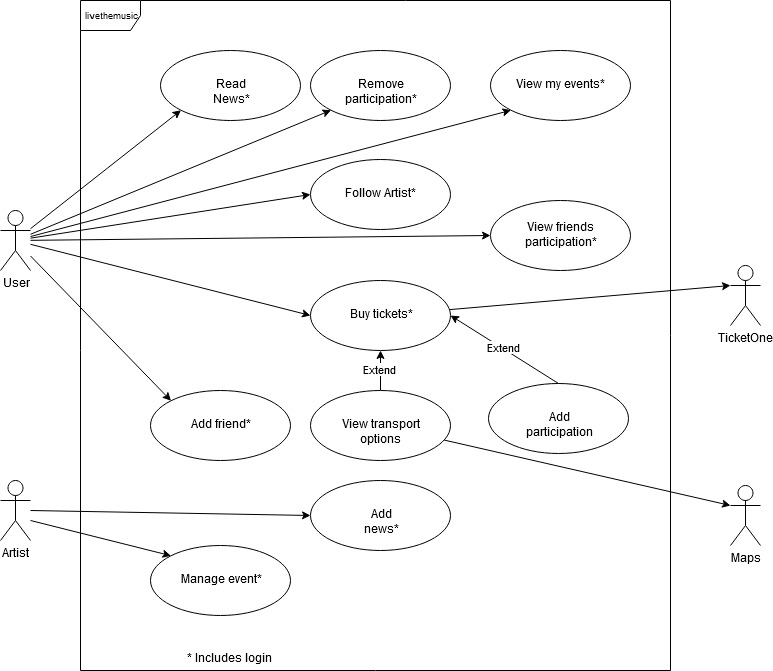
\includegraphics[scale=0.7]{UseCaseFinal.jpg}
\section{Storyboard}
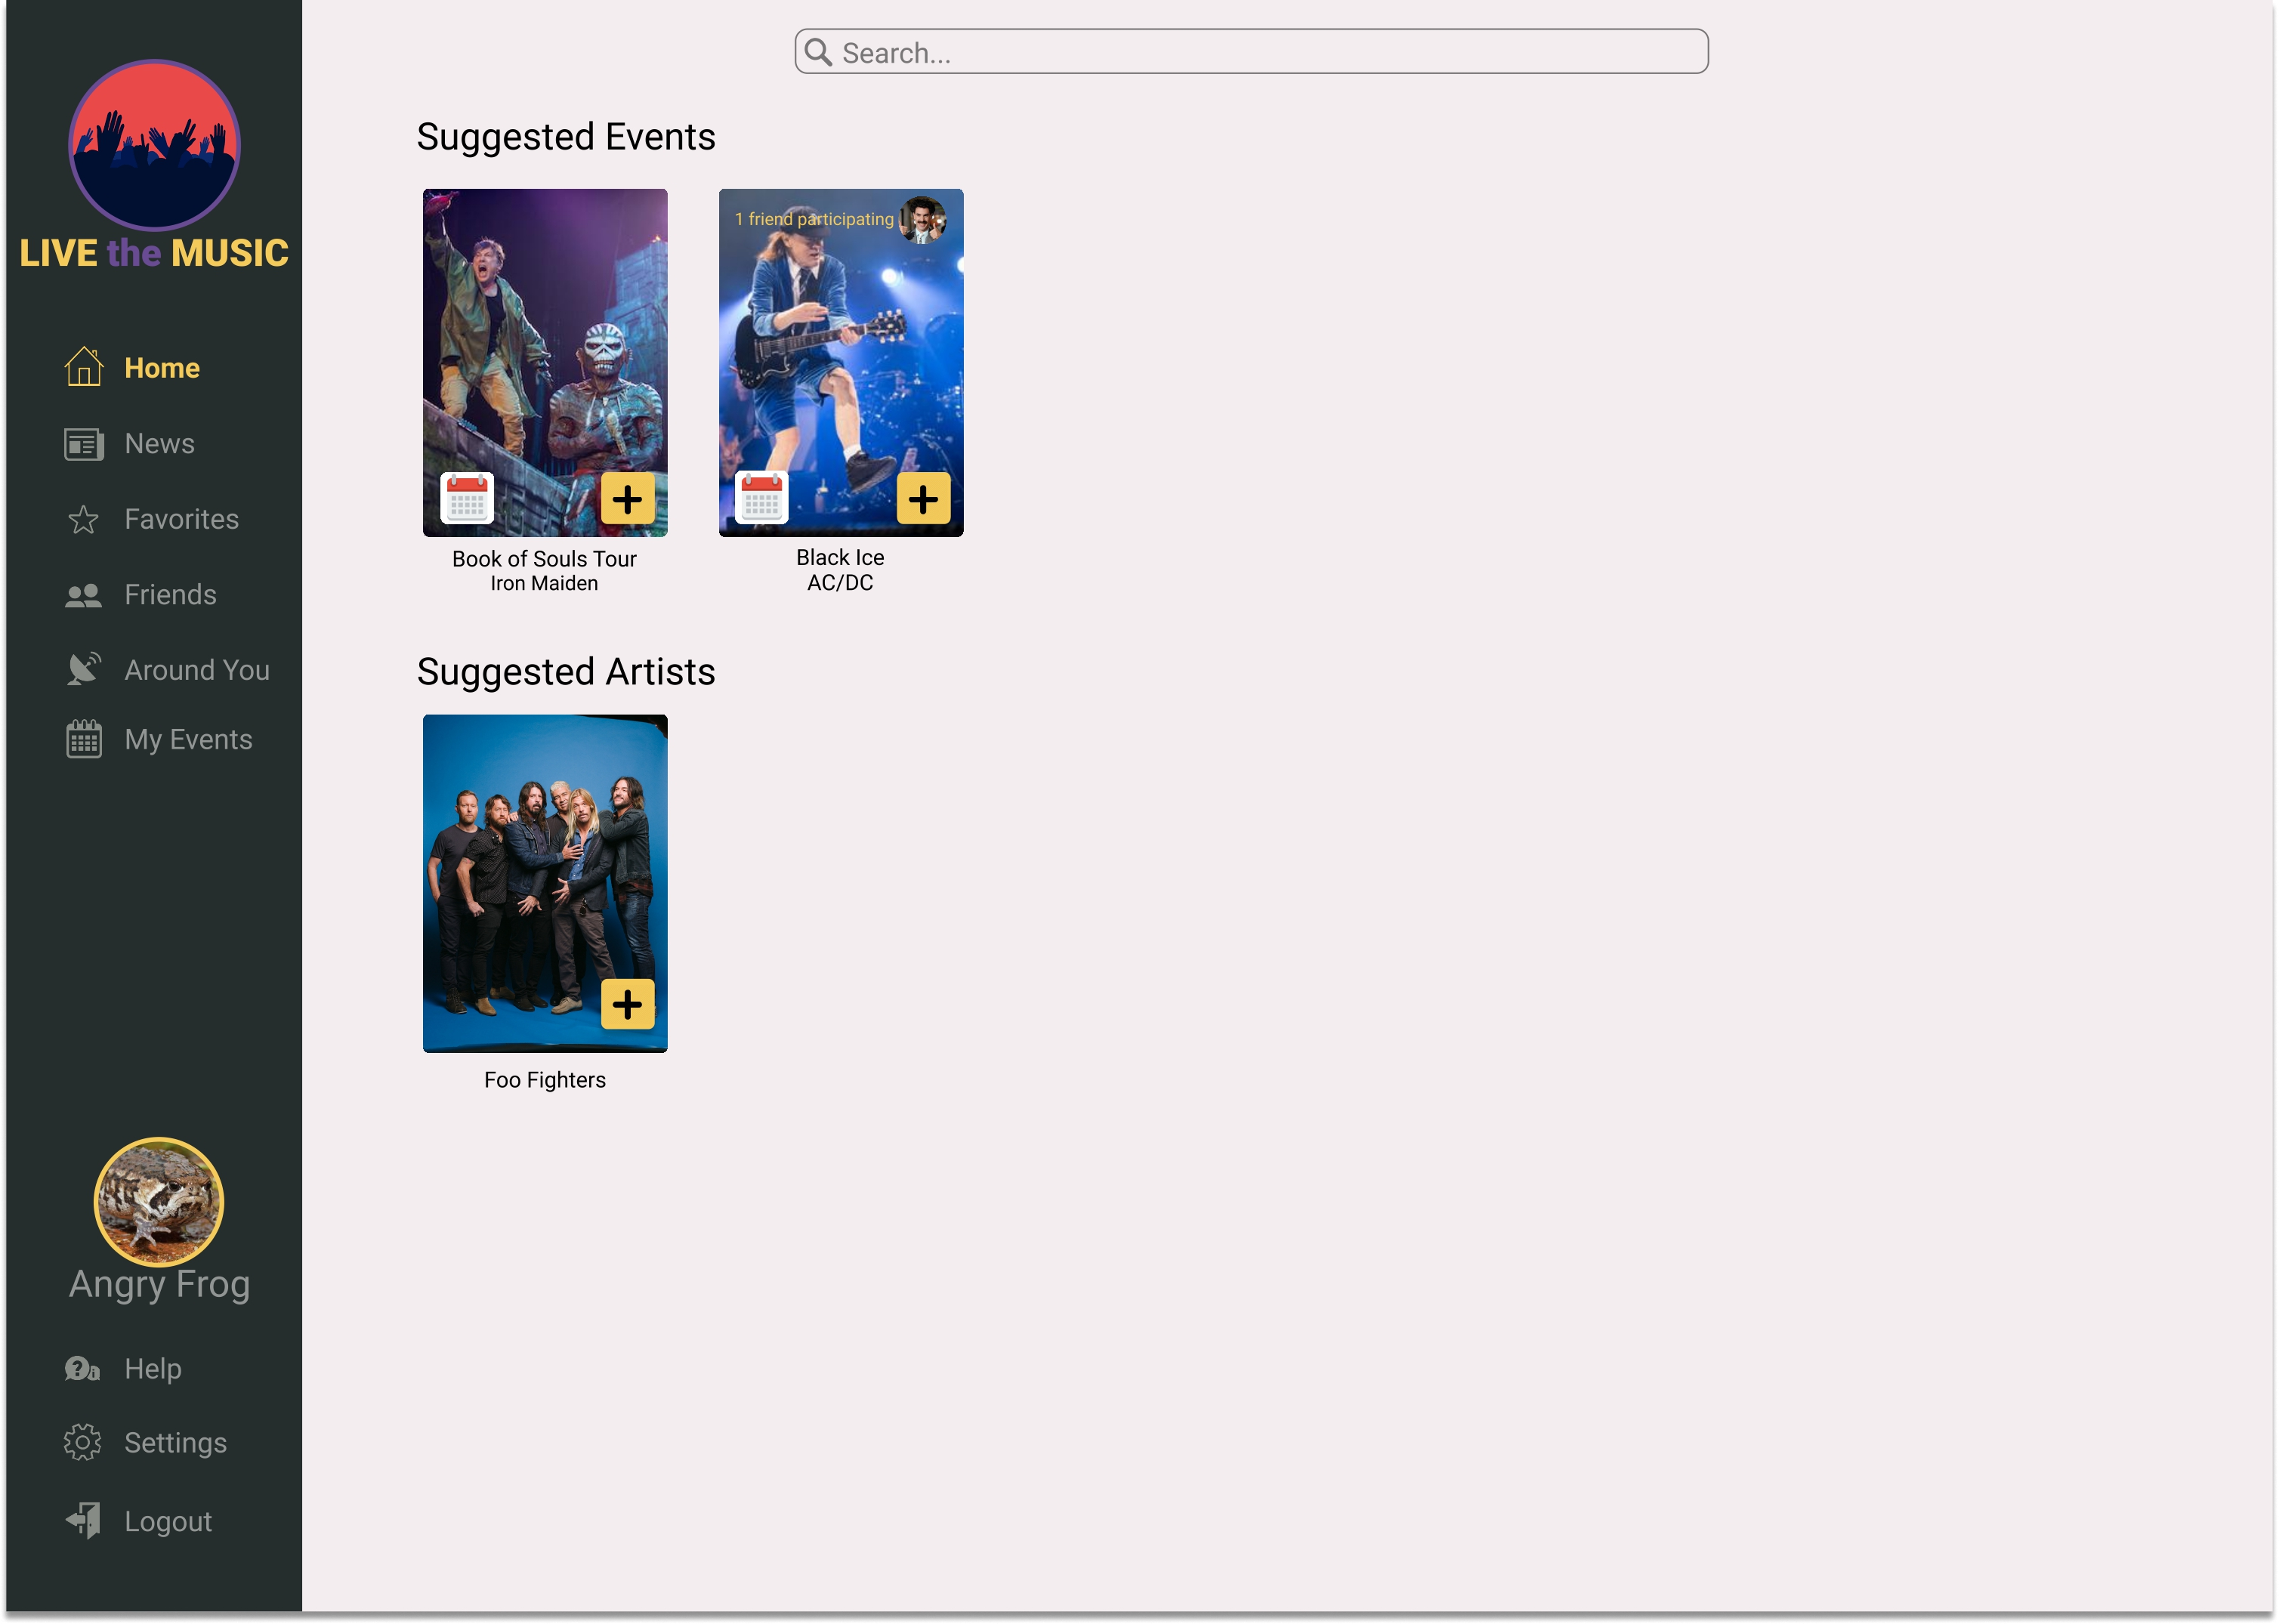
\includegraphics[scale=0.25]{Home.jpg}
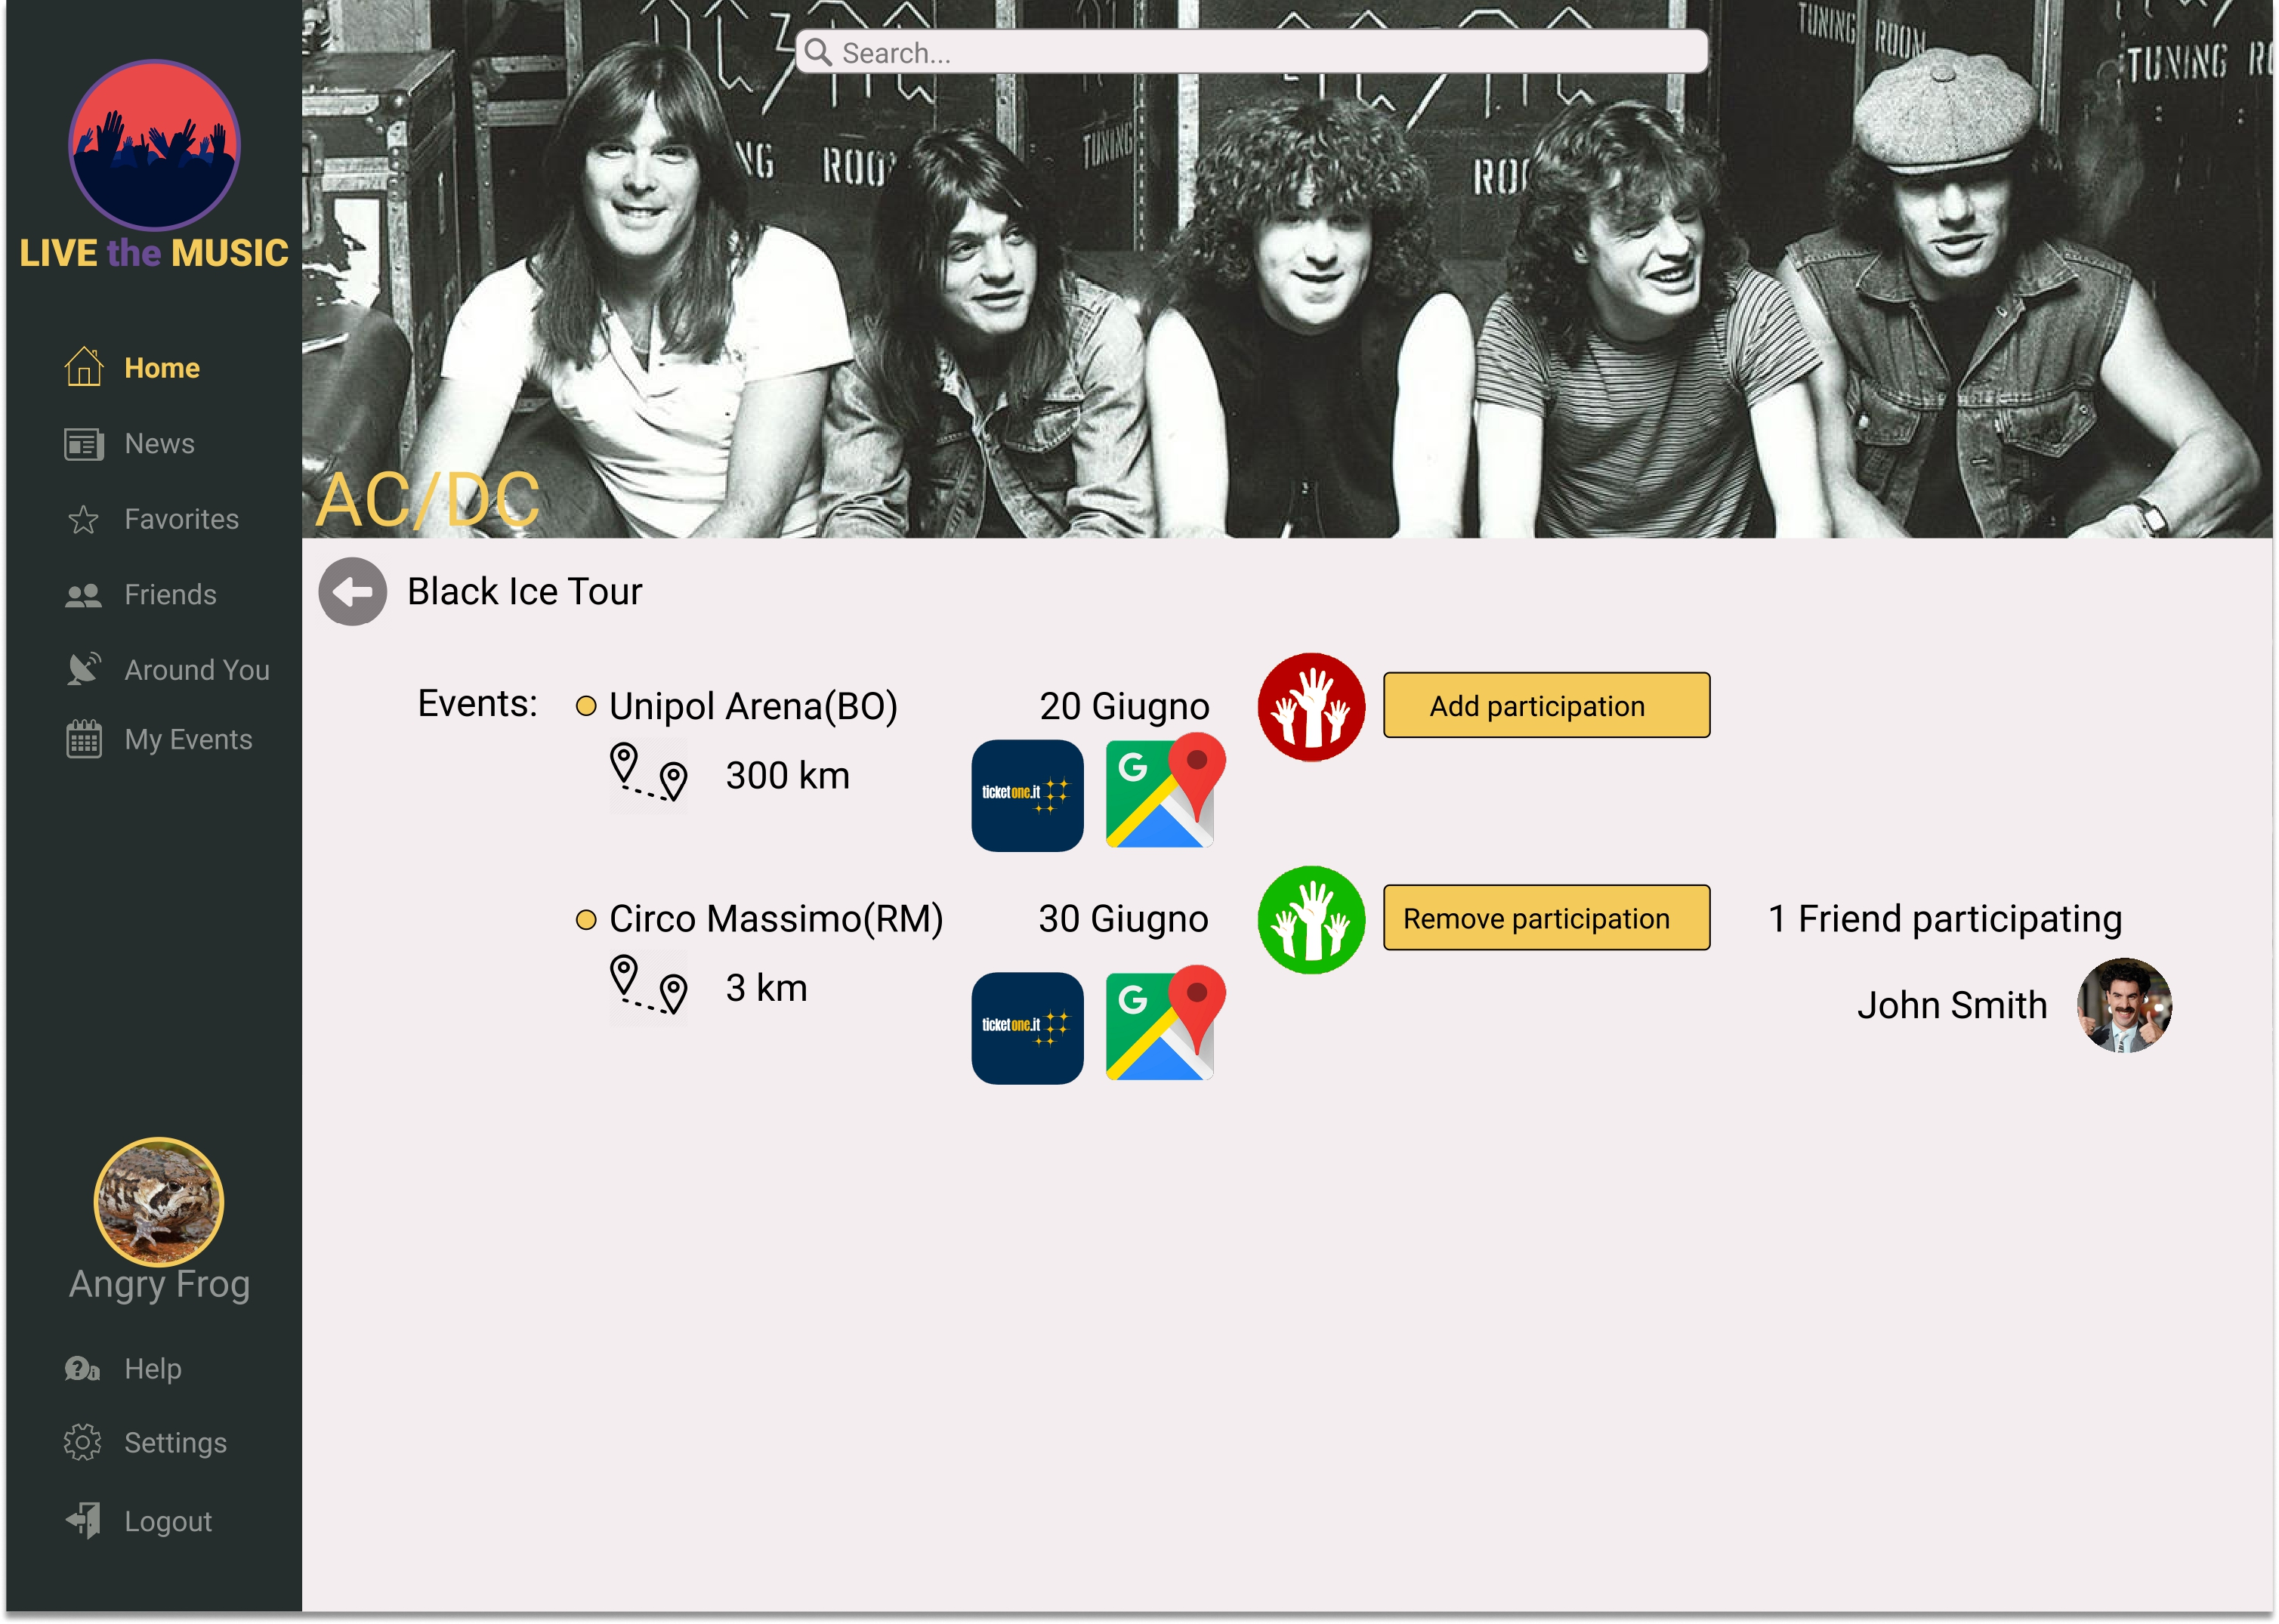
\includegraphics[scale=0.25]{Concert.jpg}
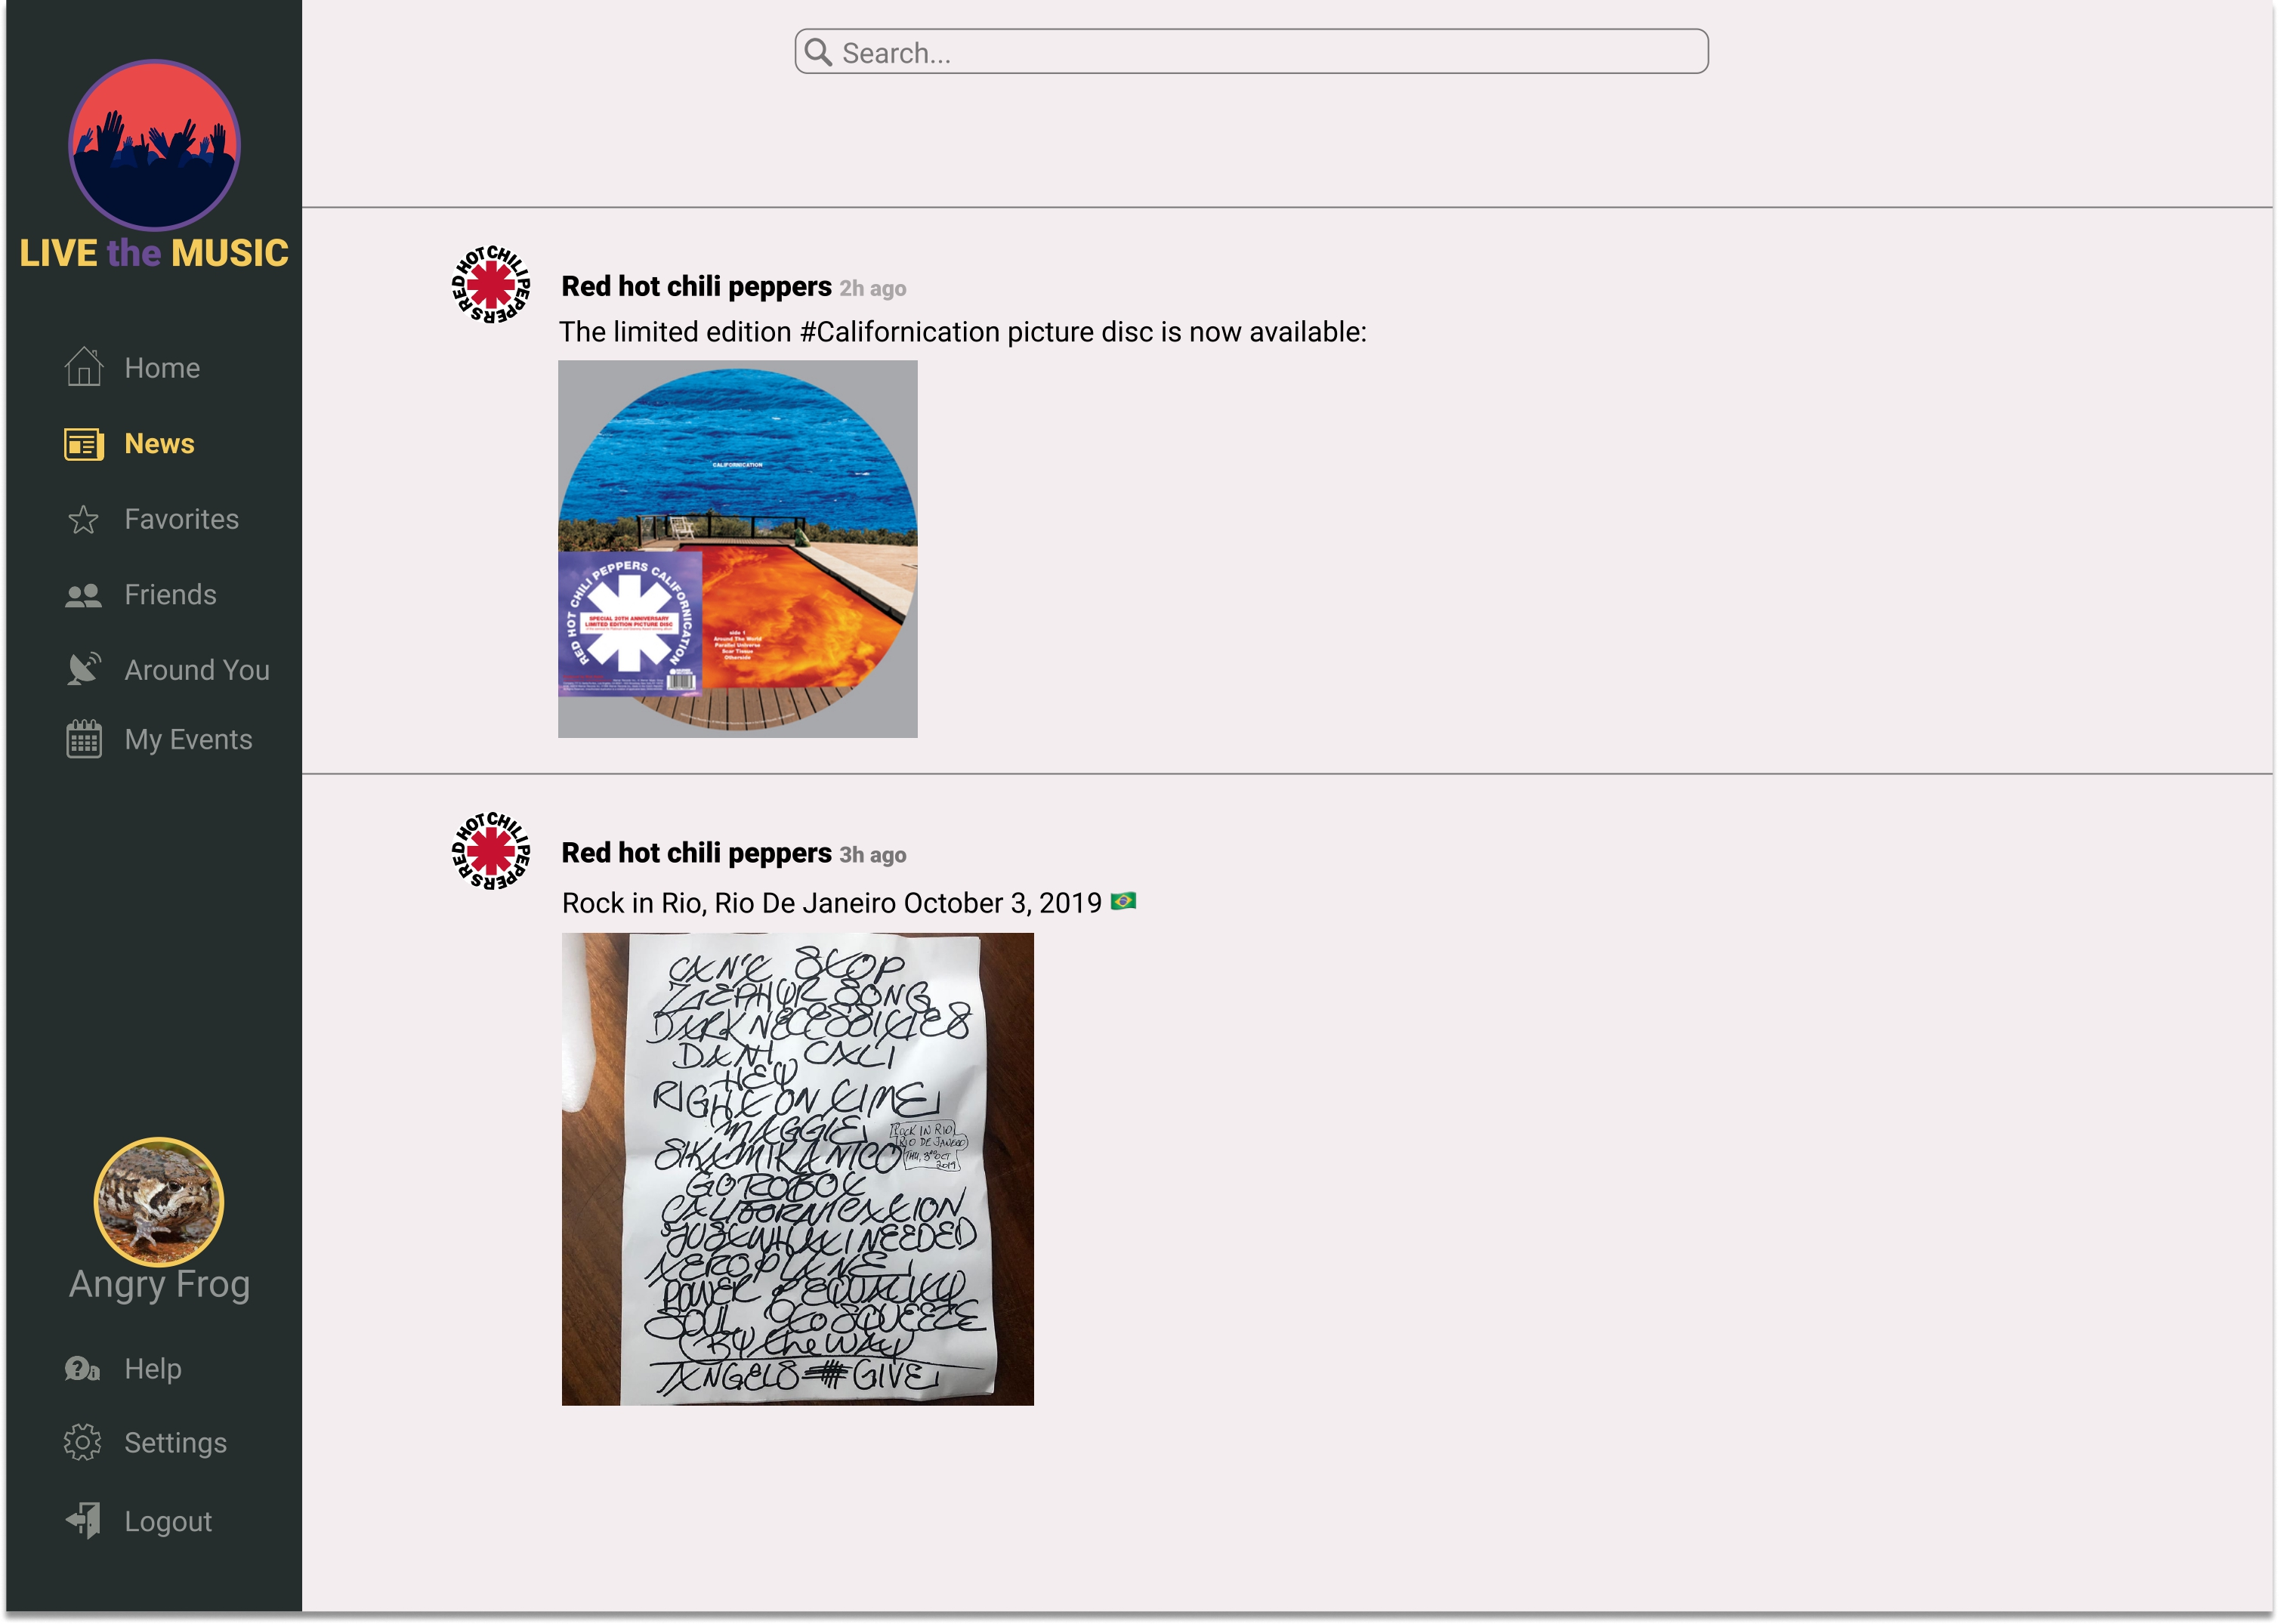
\includegraphics[scale=0.25]{News.jpg}
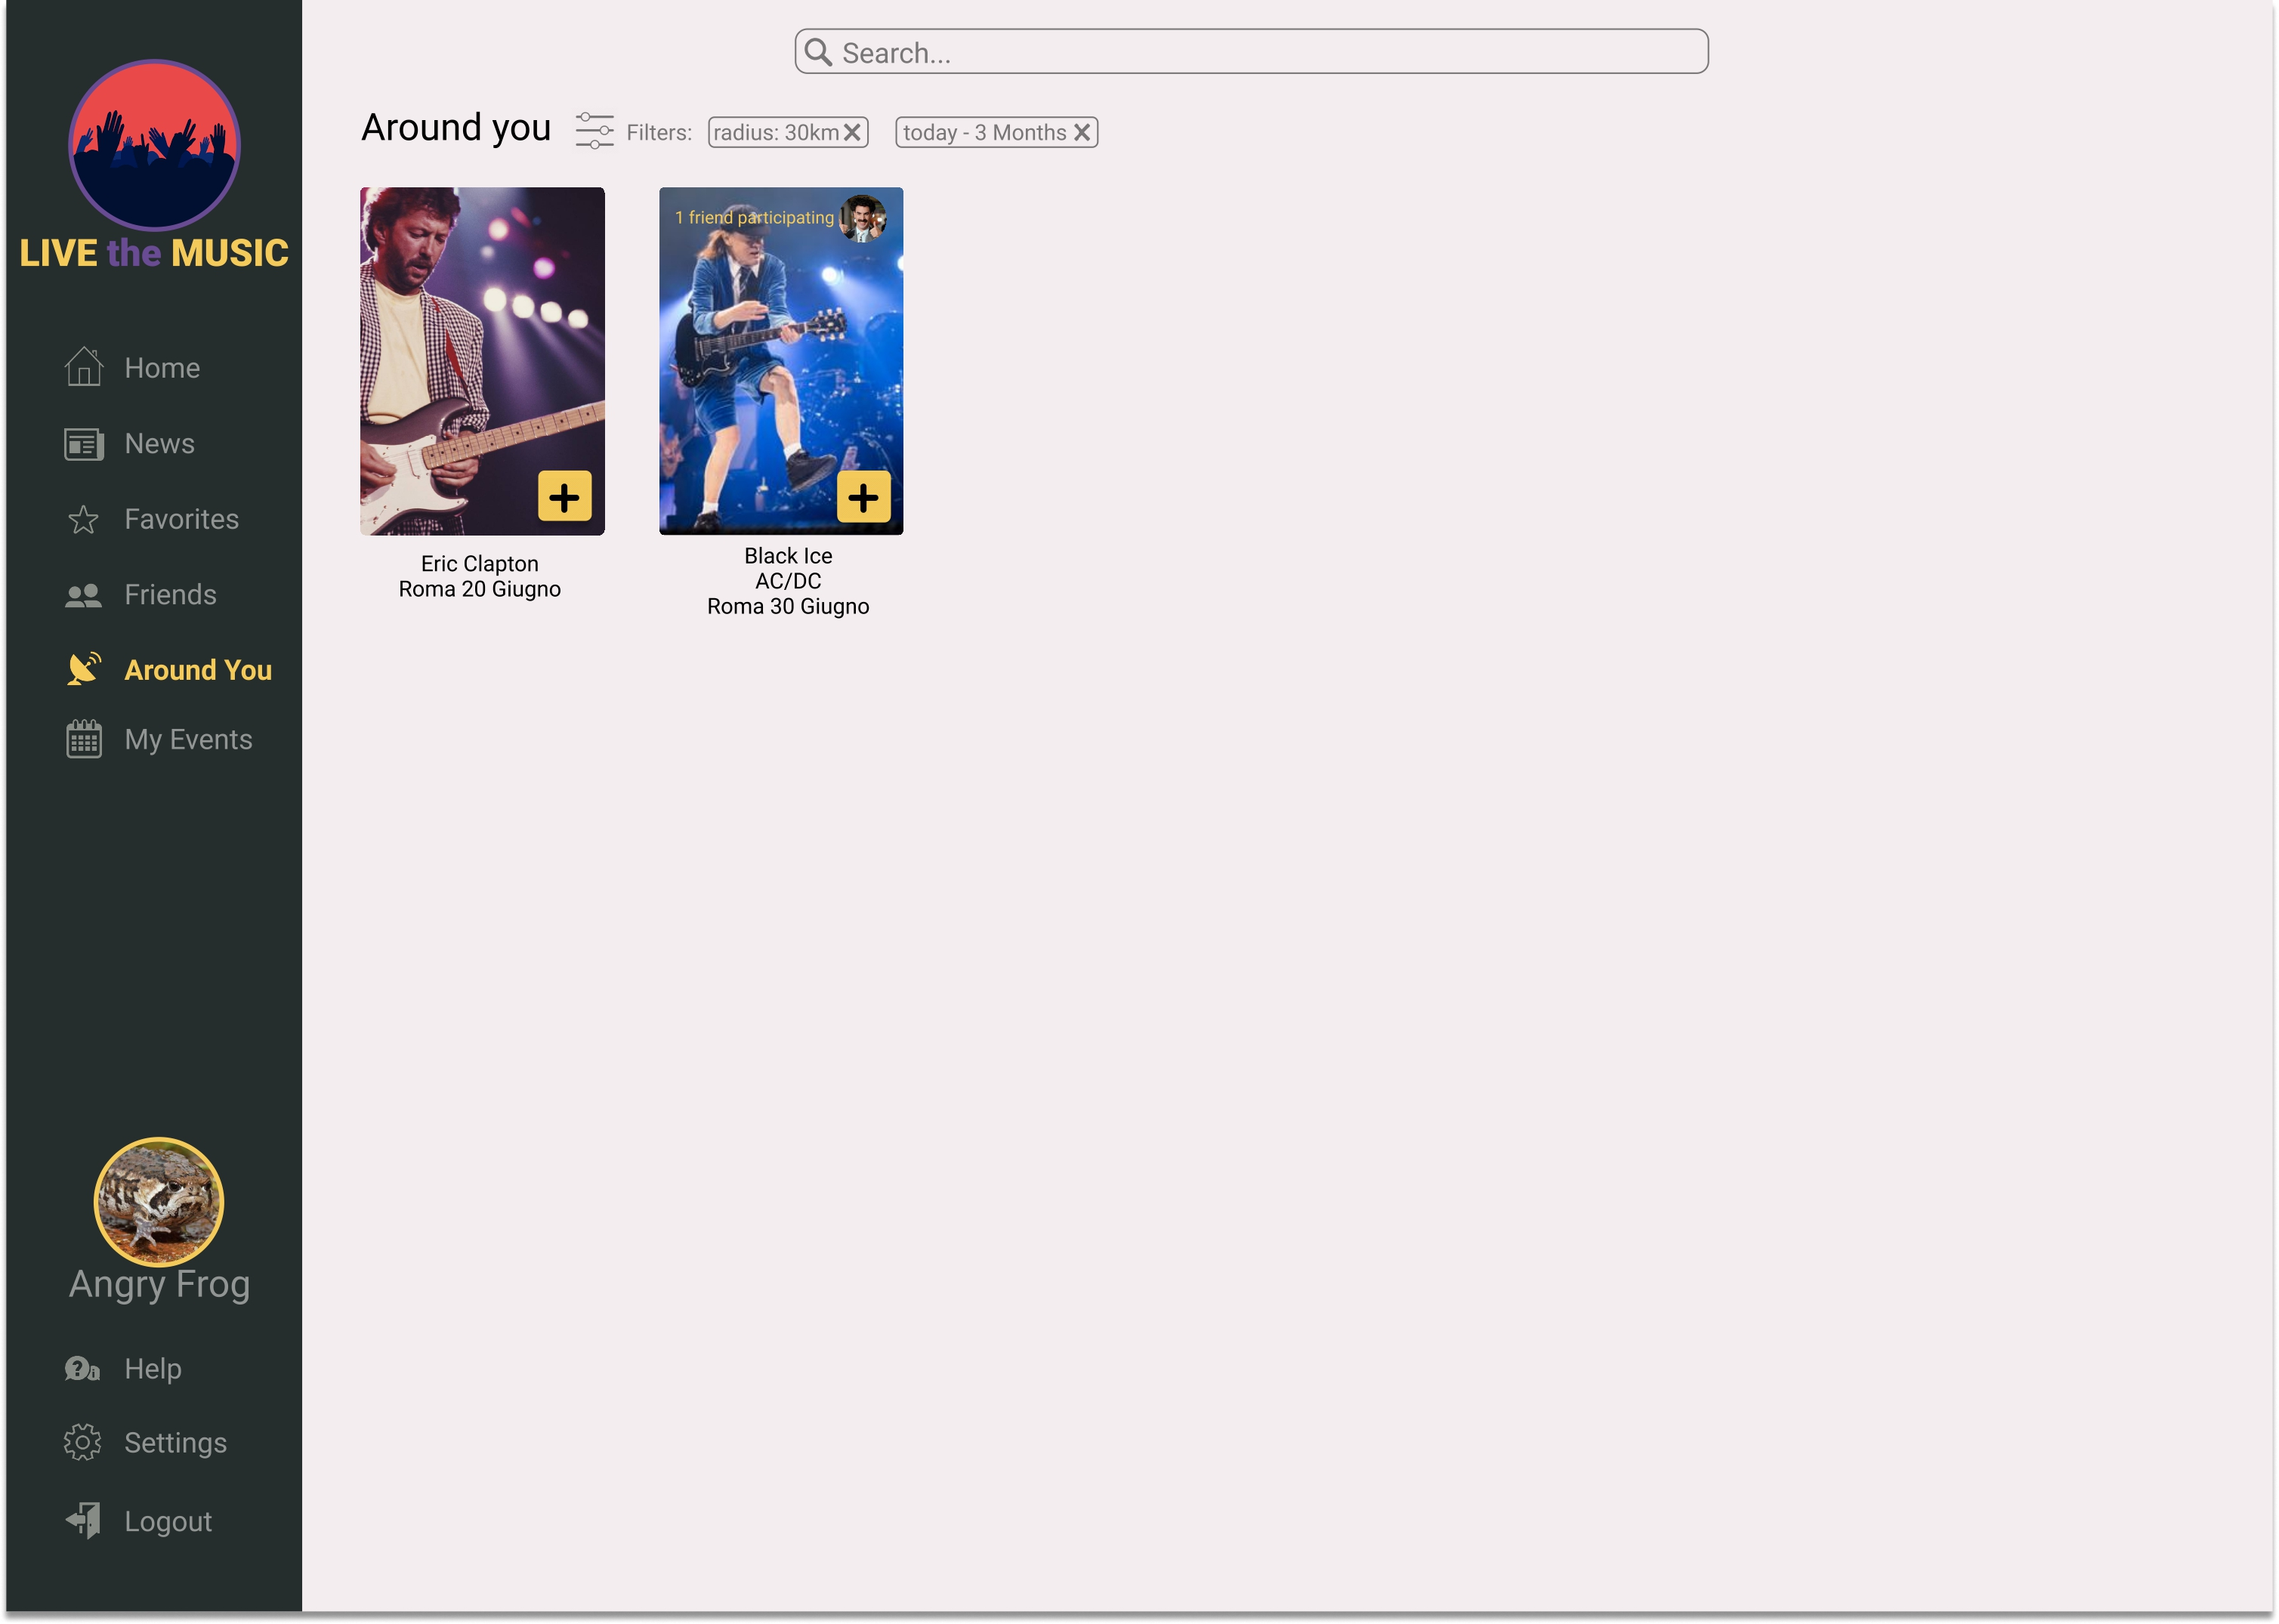
\includegraphics[scale=0.25]{AroundYou.jpg}
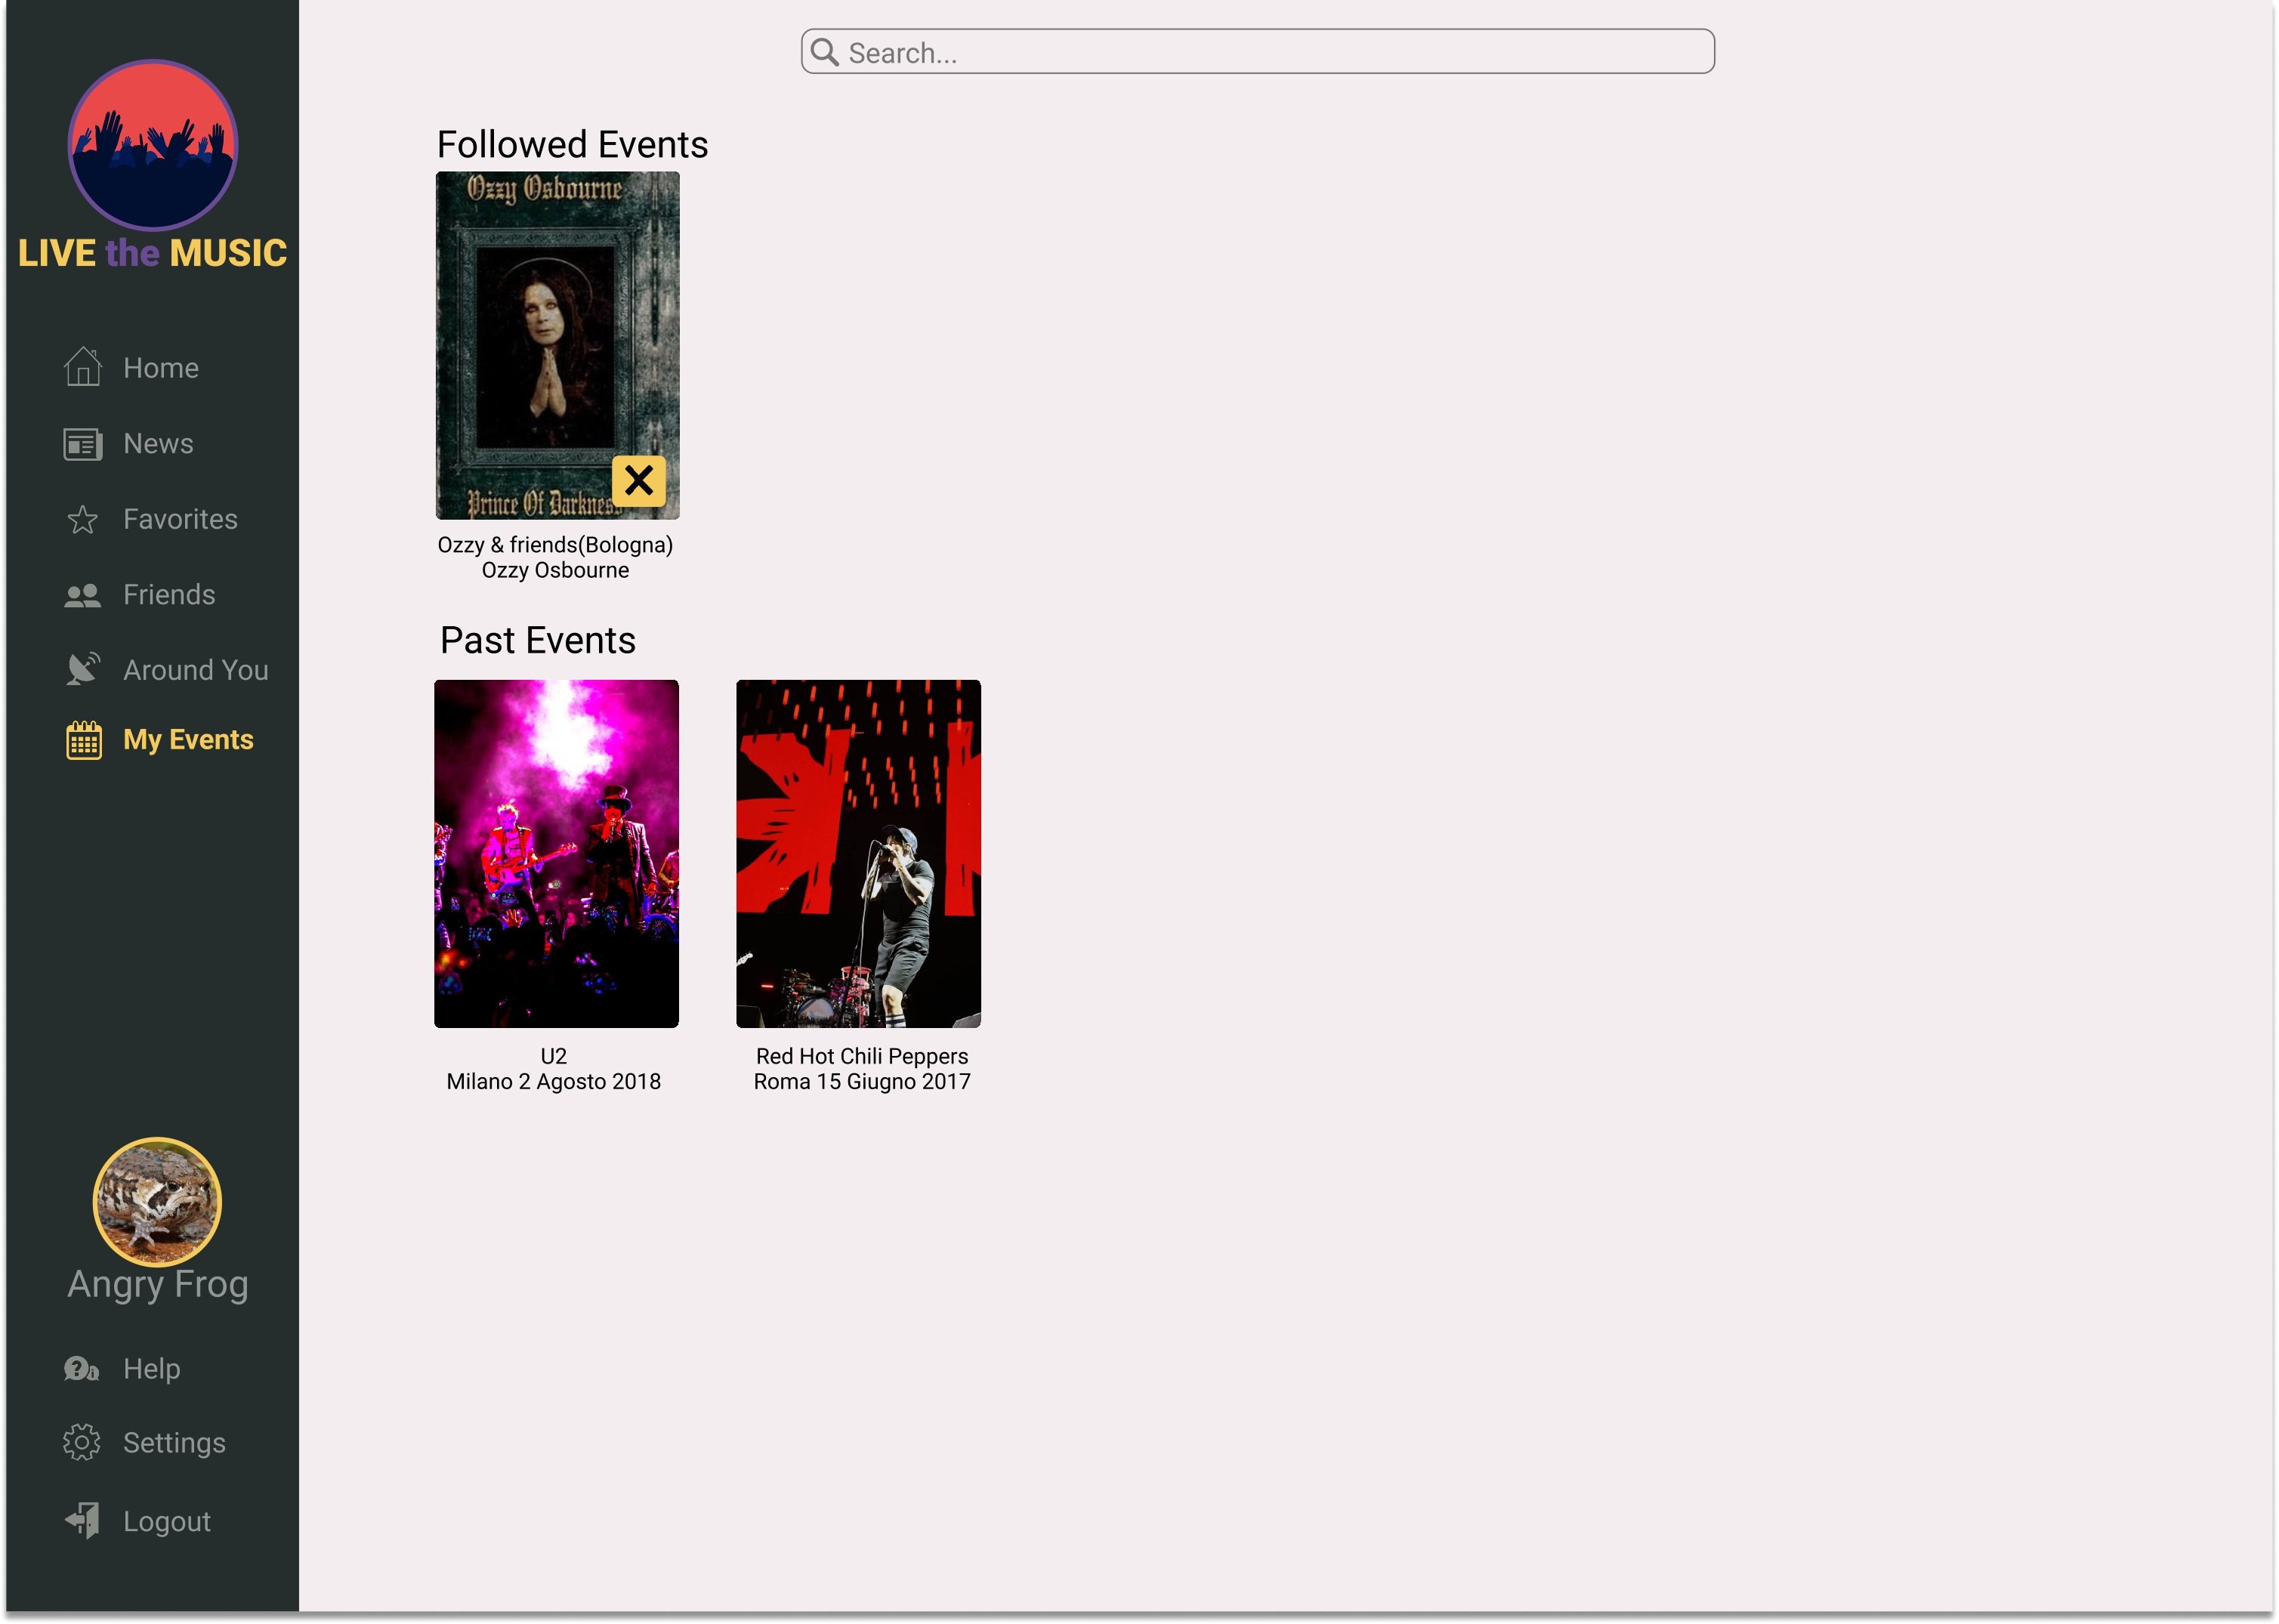
\includegraphics[scale=0.25]{MyEvents.jpg}
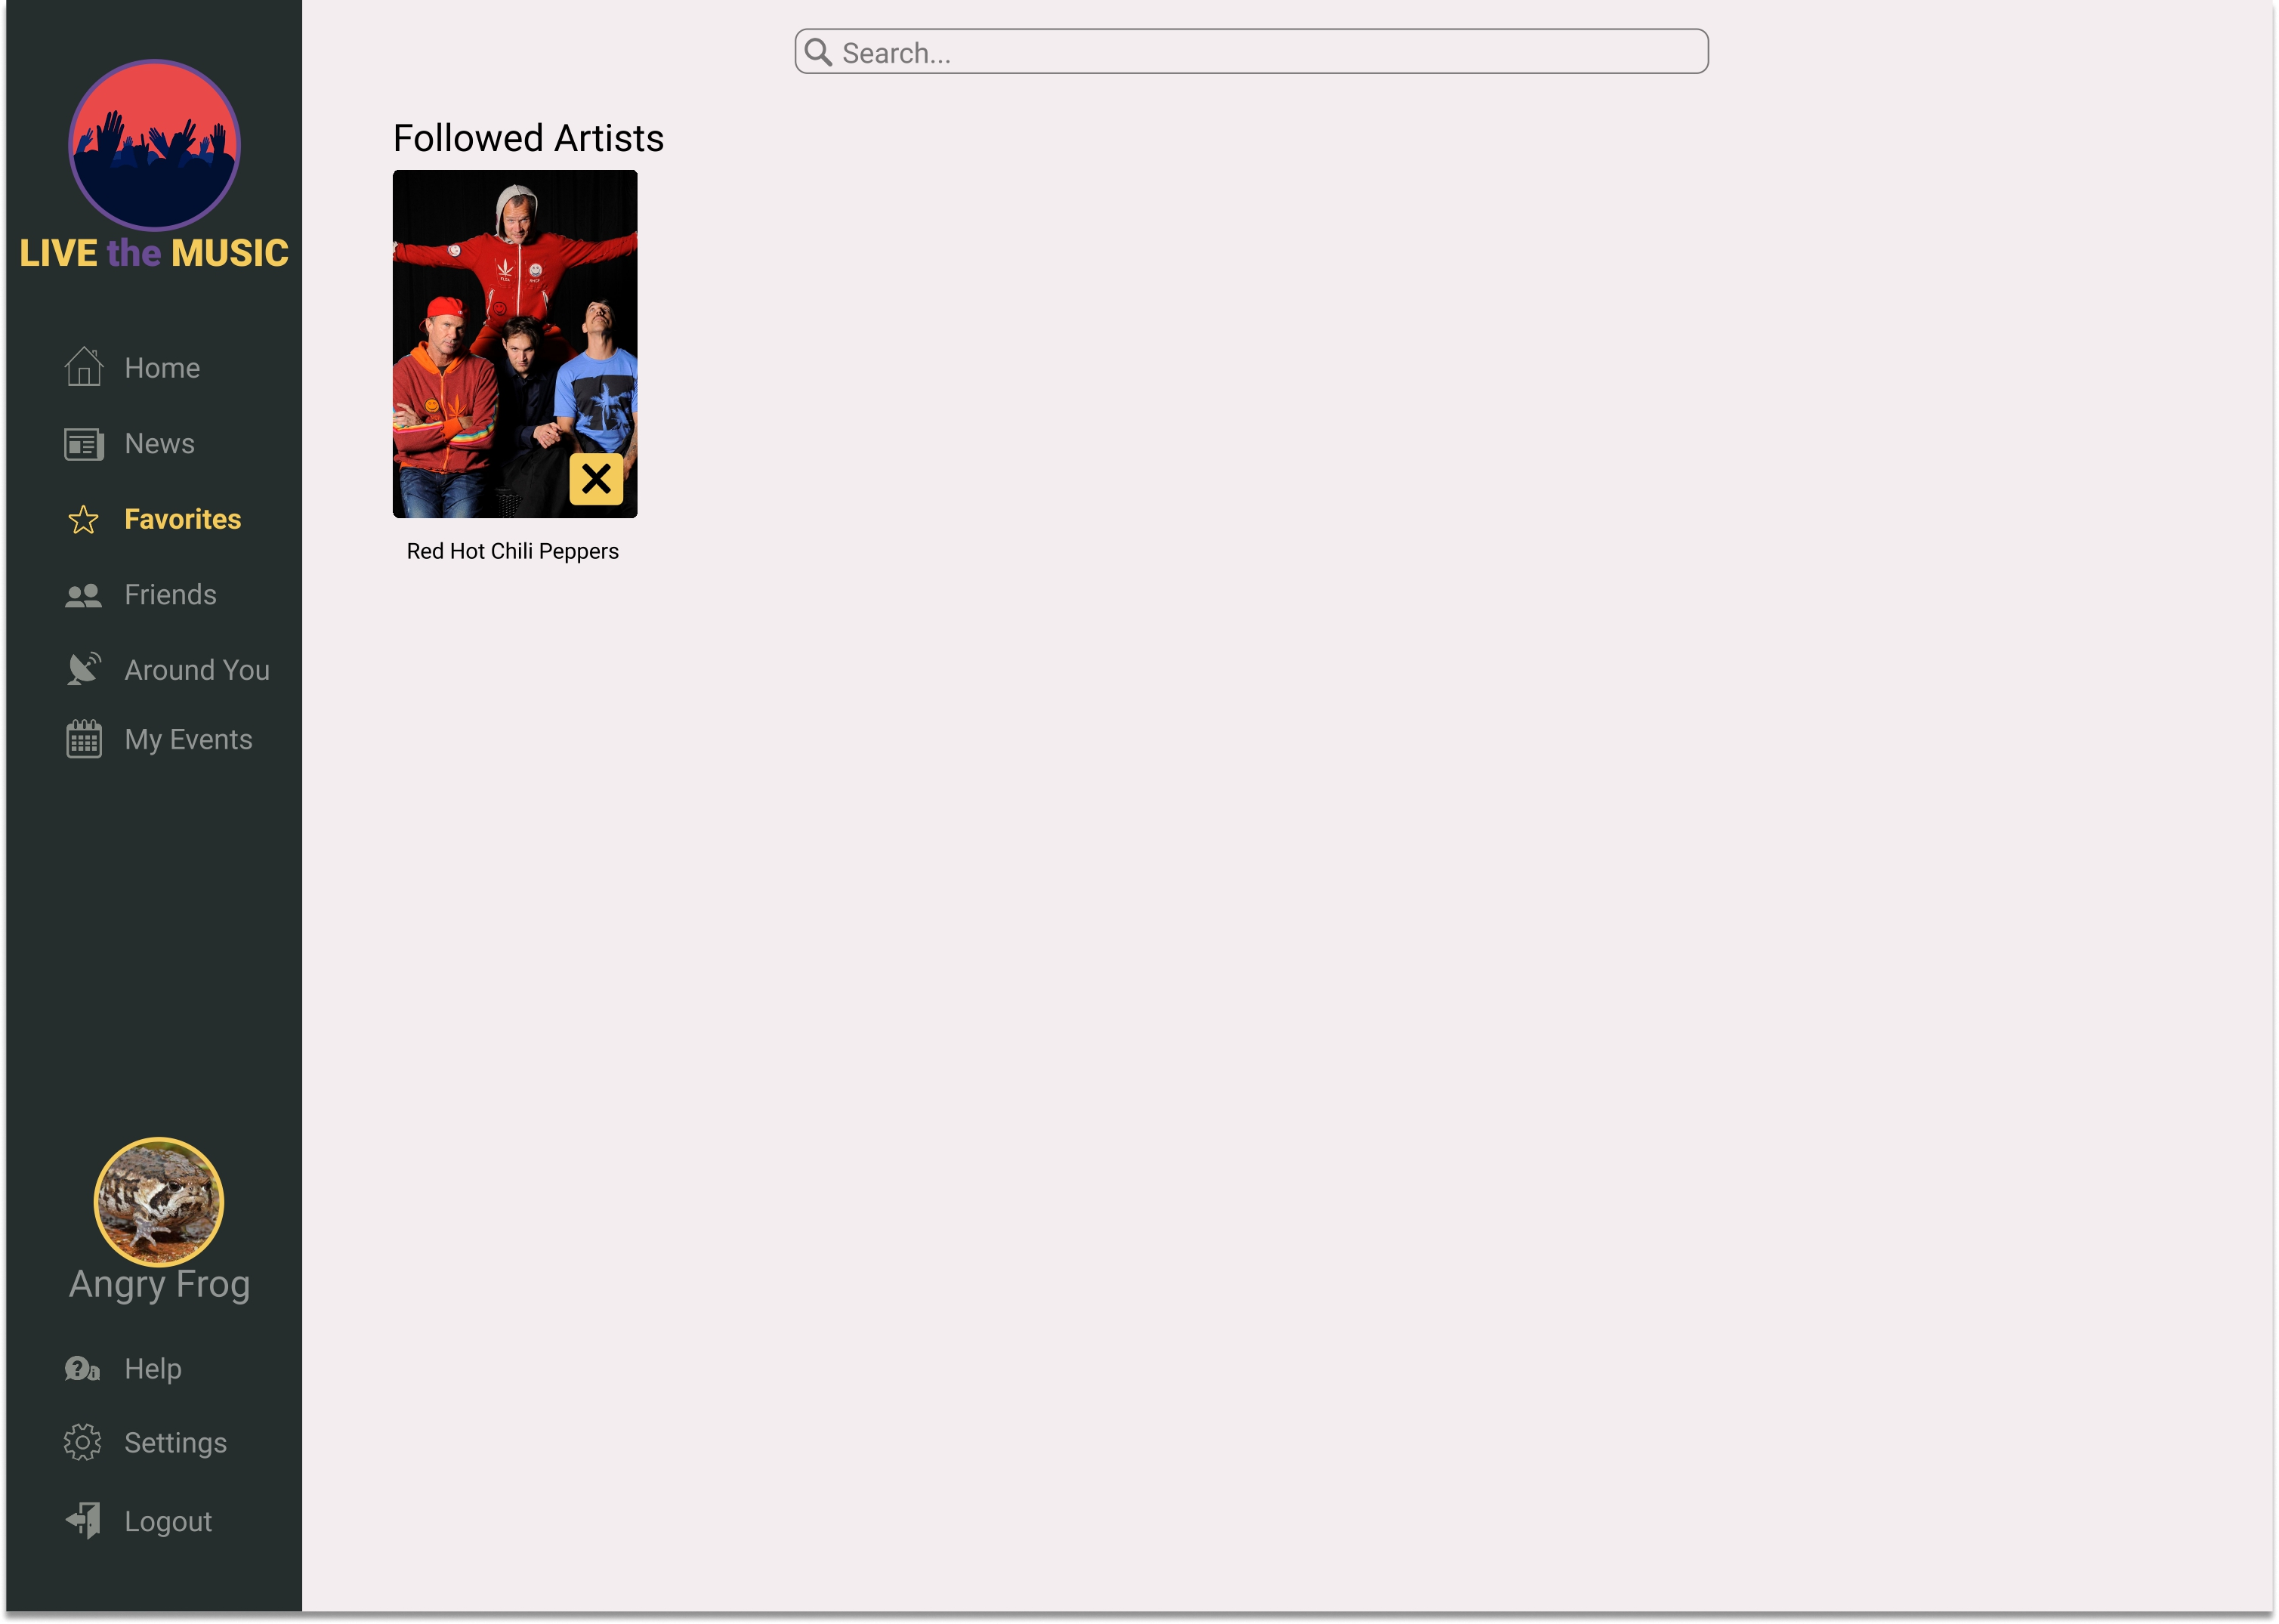
\includegraphics[scale=0.25]{Favorites.jpg}
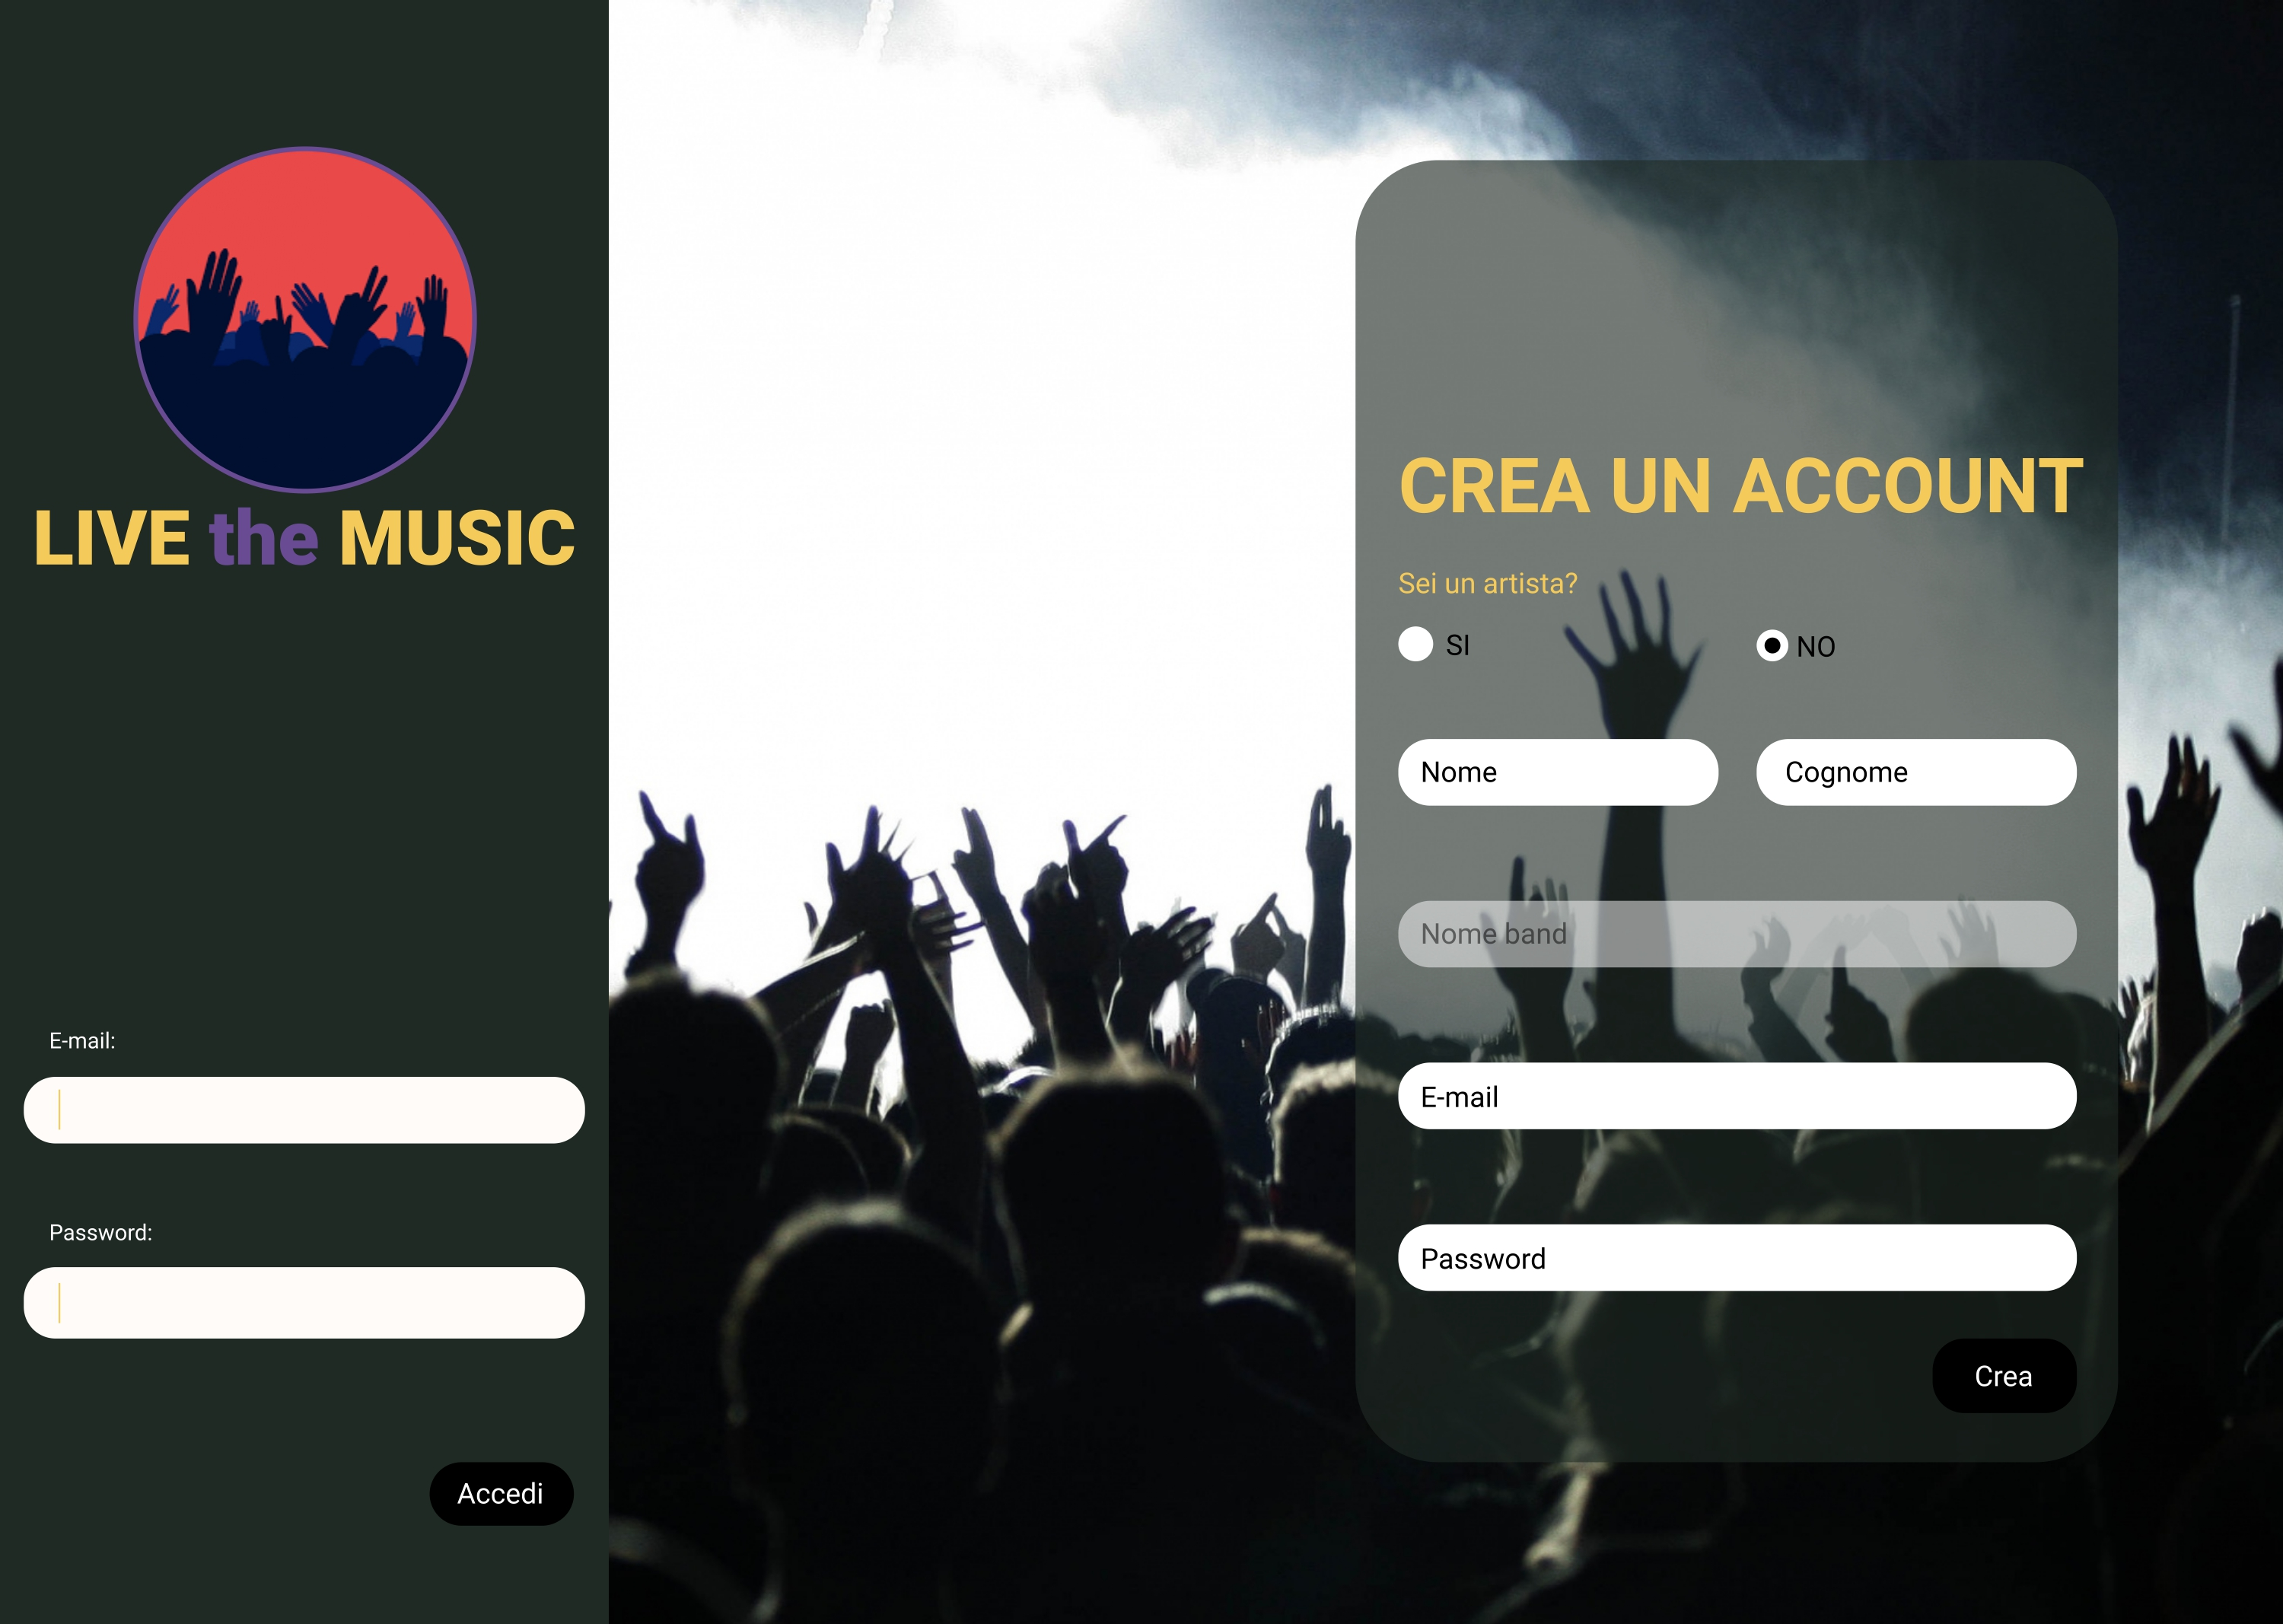
\includegraphics[scale=0.25]{Login.jpg}
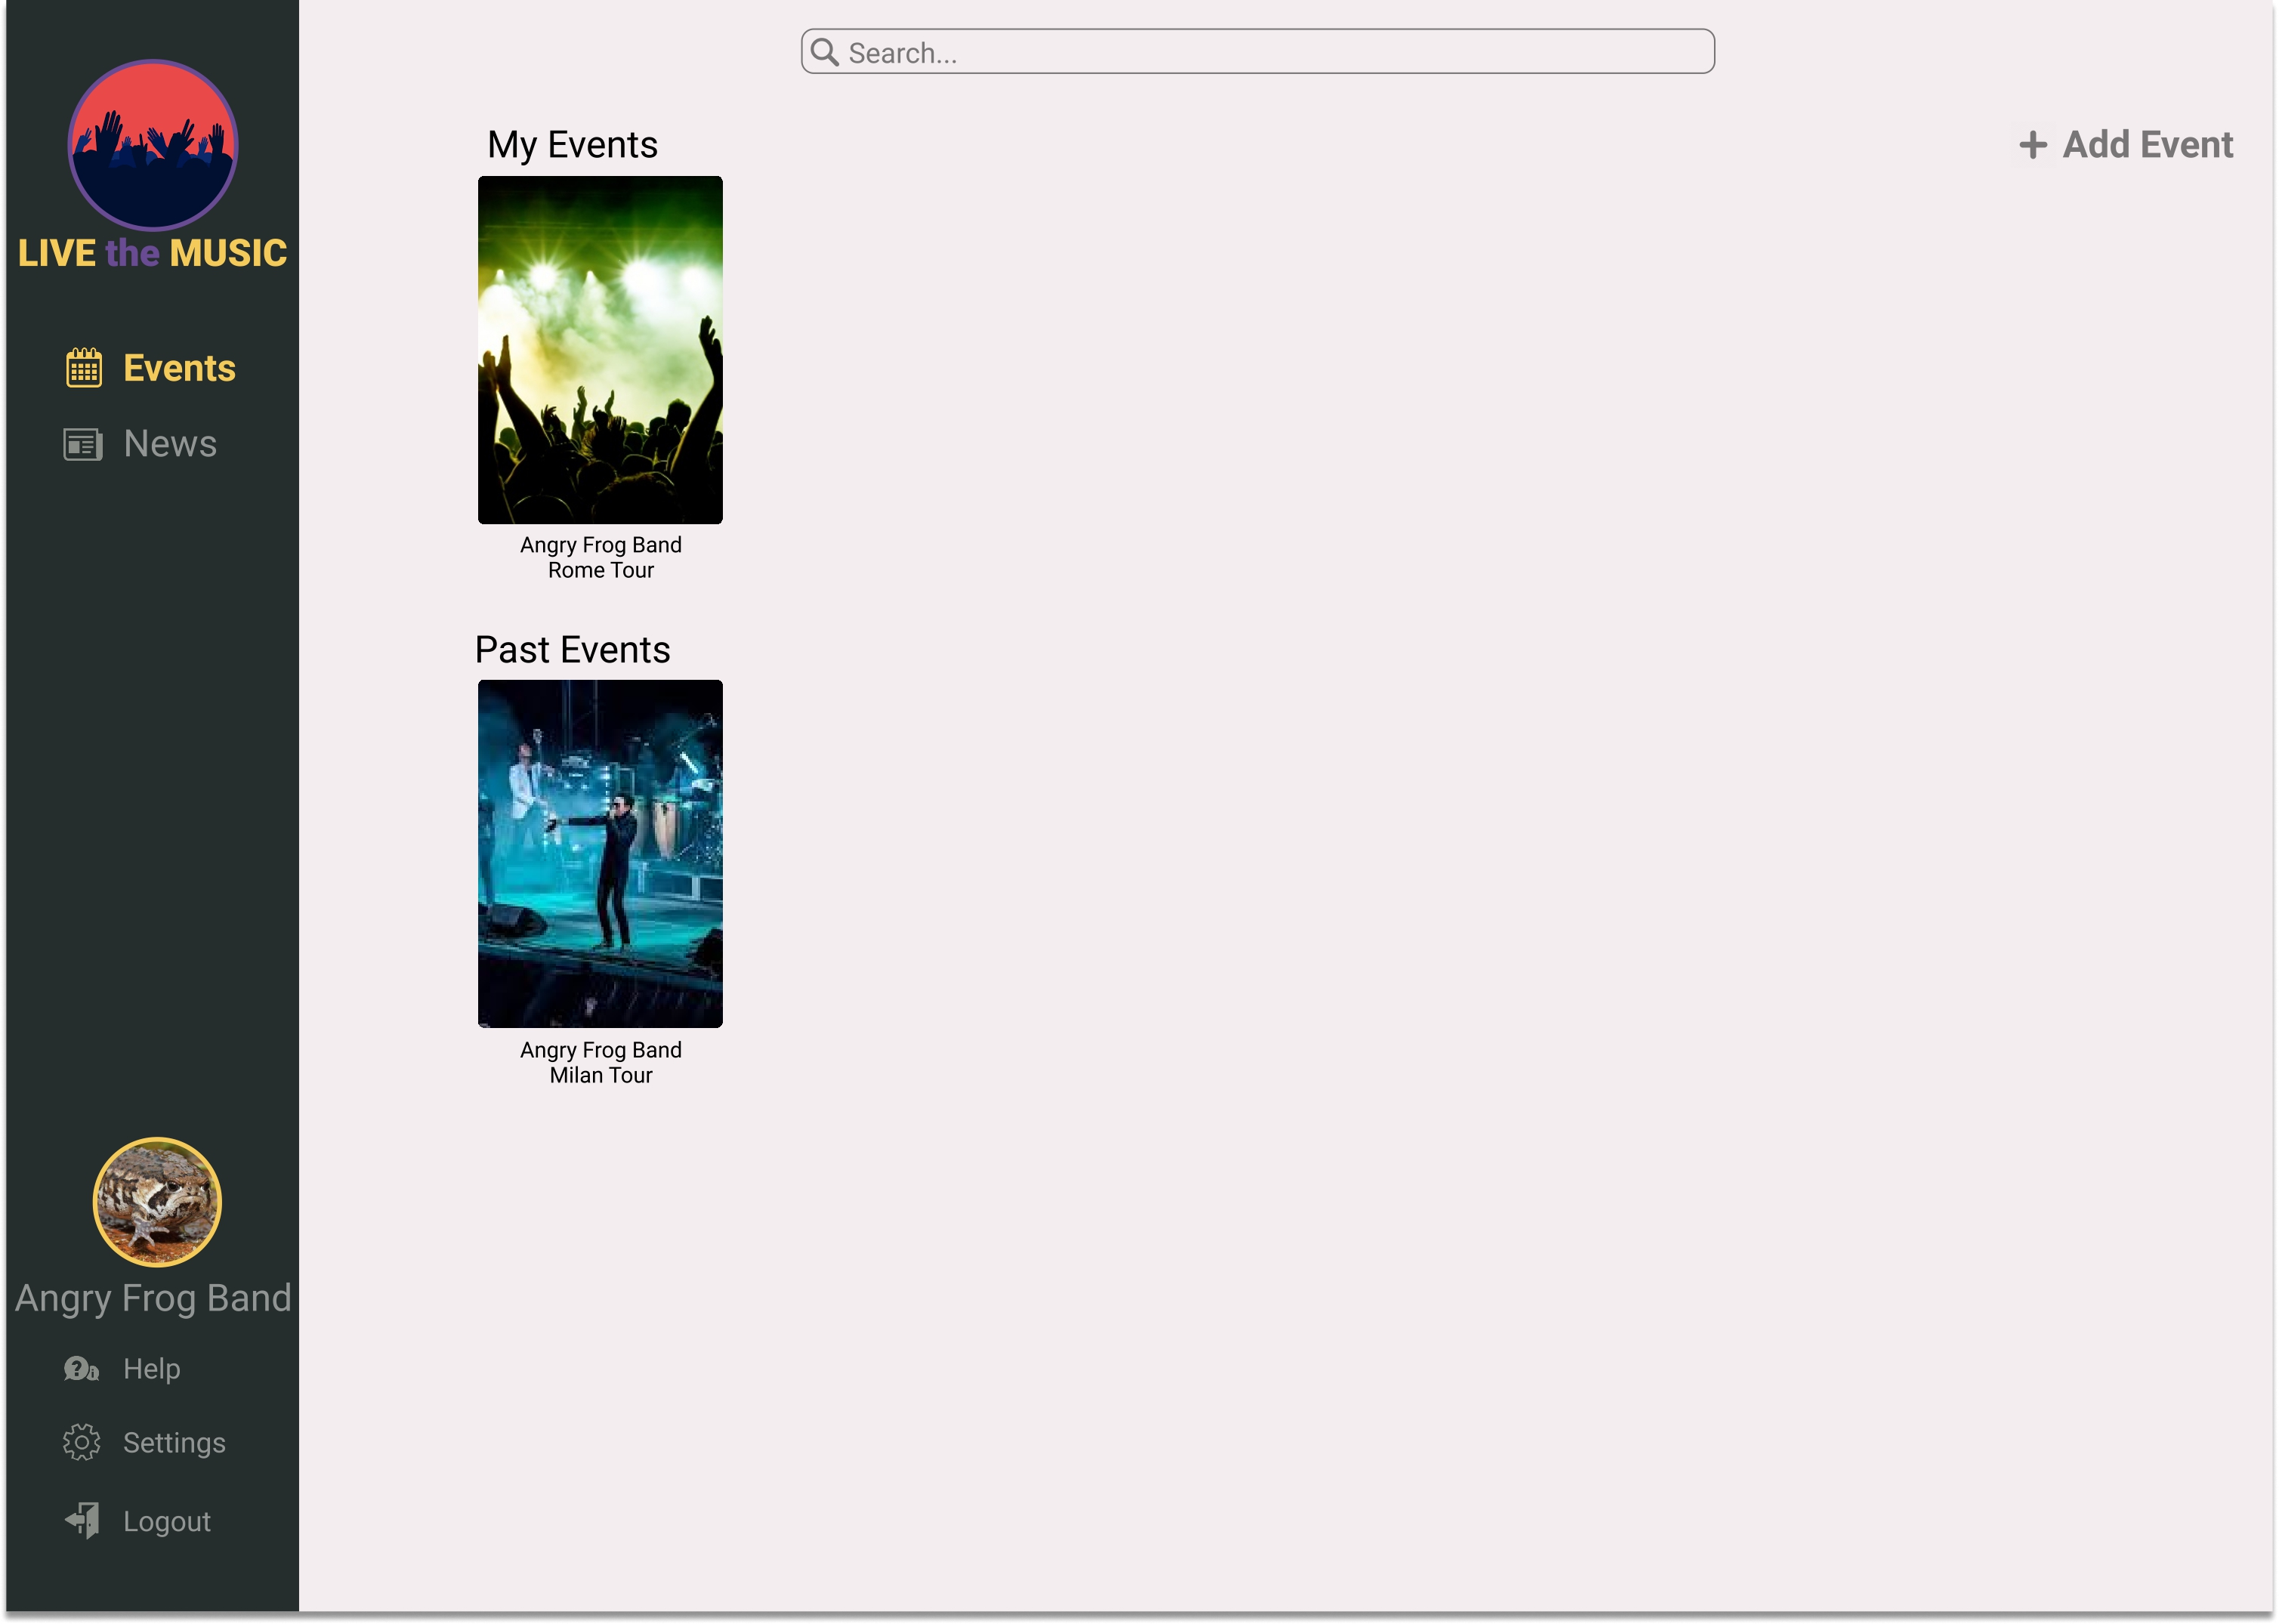
\includegraphics[scale=0.25]{AddEvent.jpg}
\section{Activity Diagram}
\subsection{Donato}
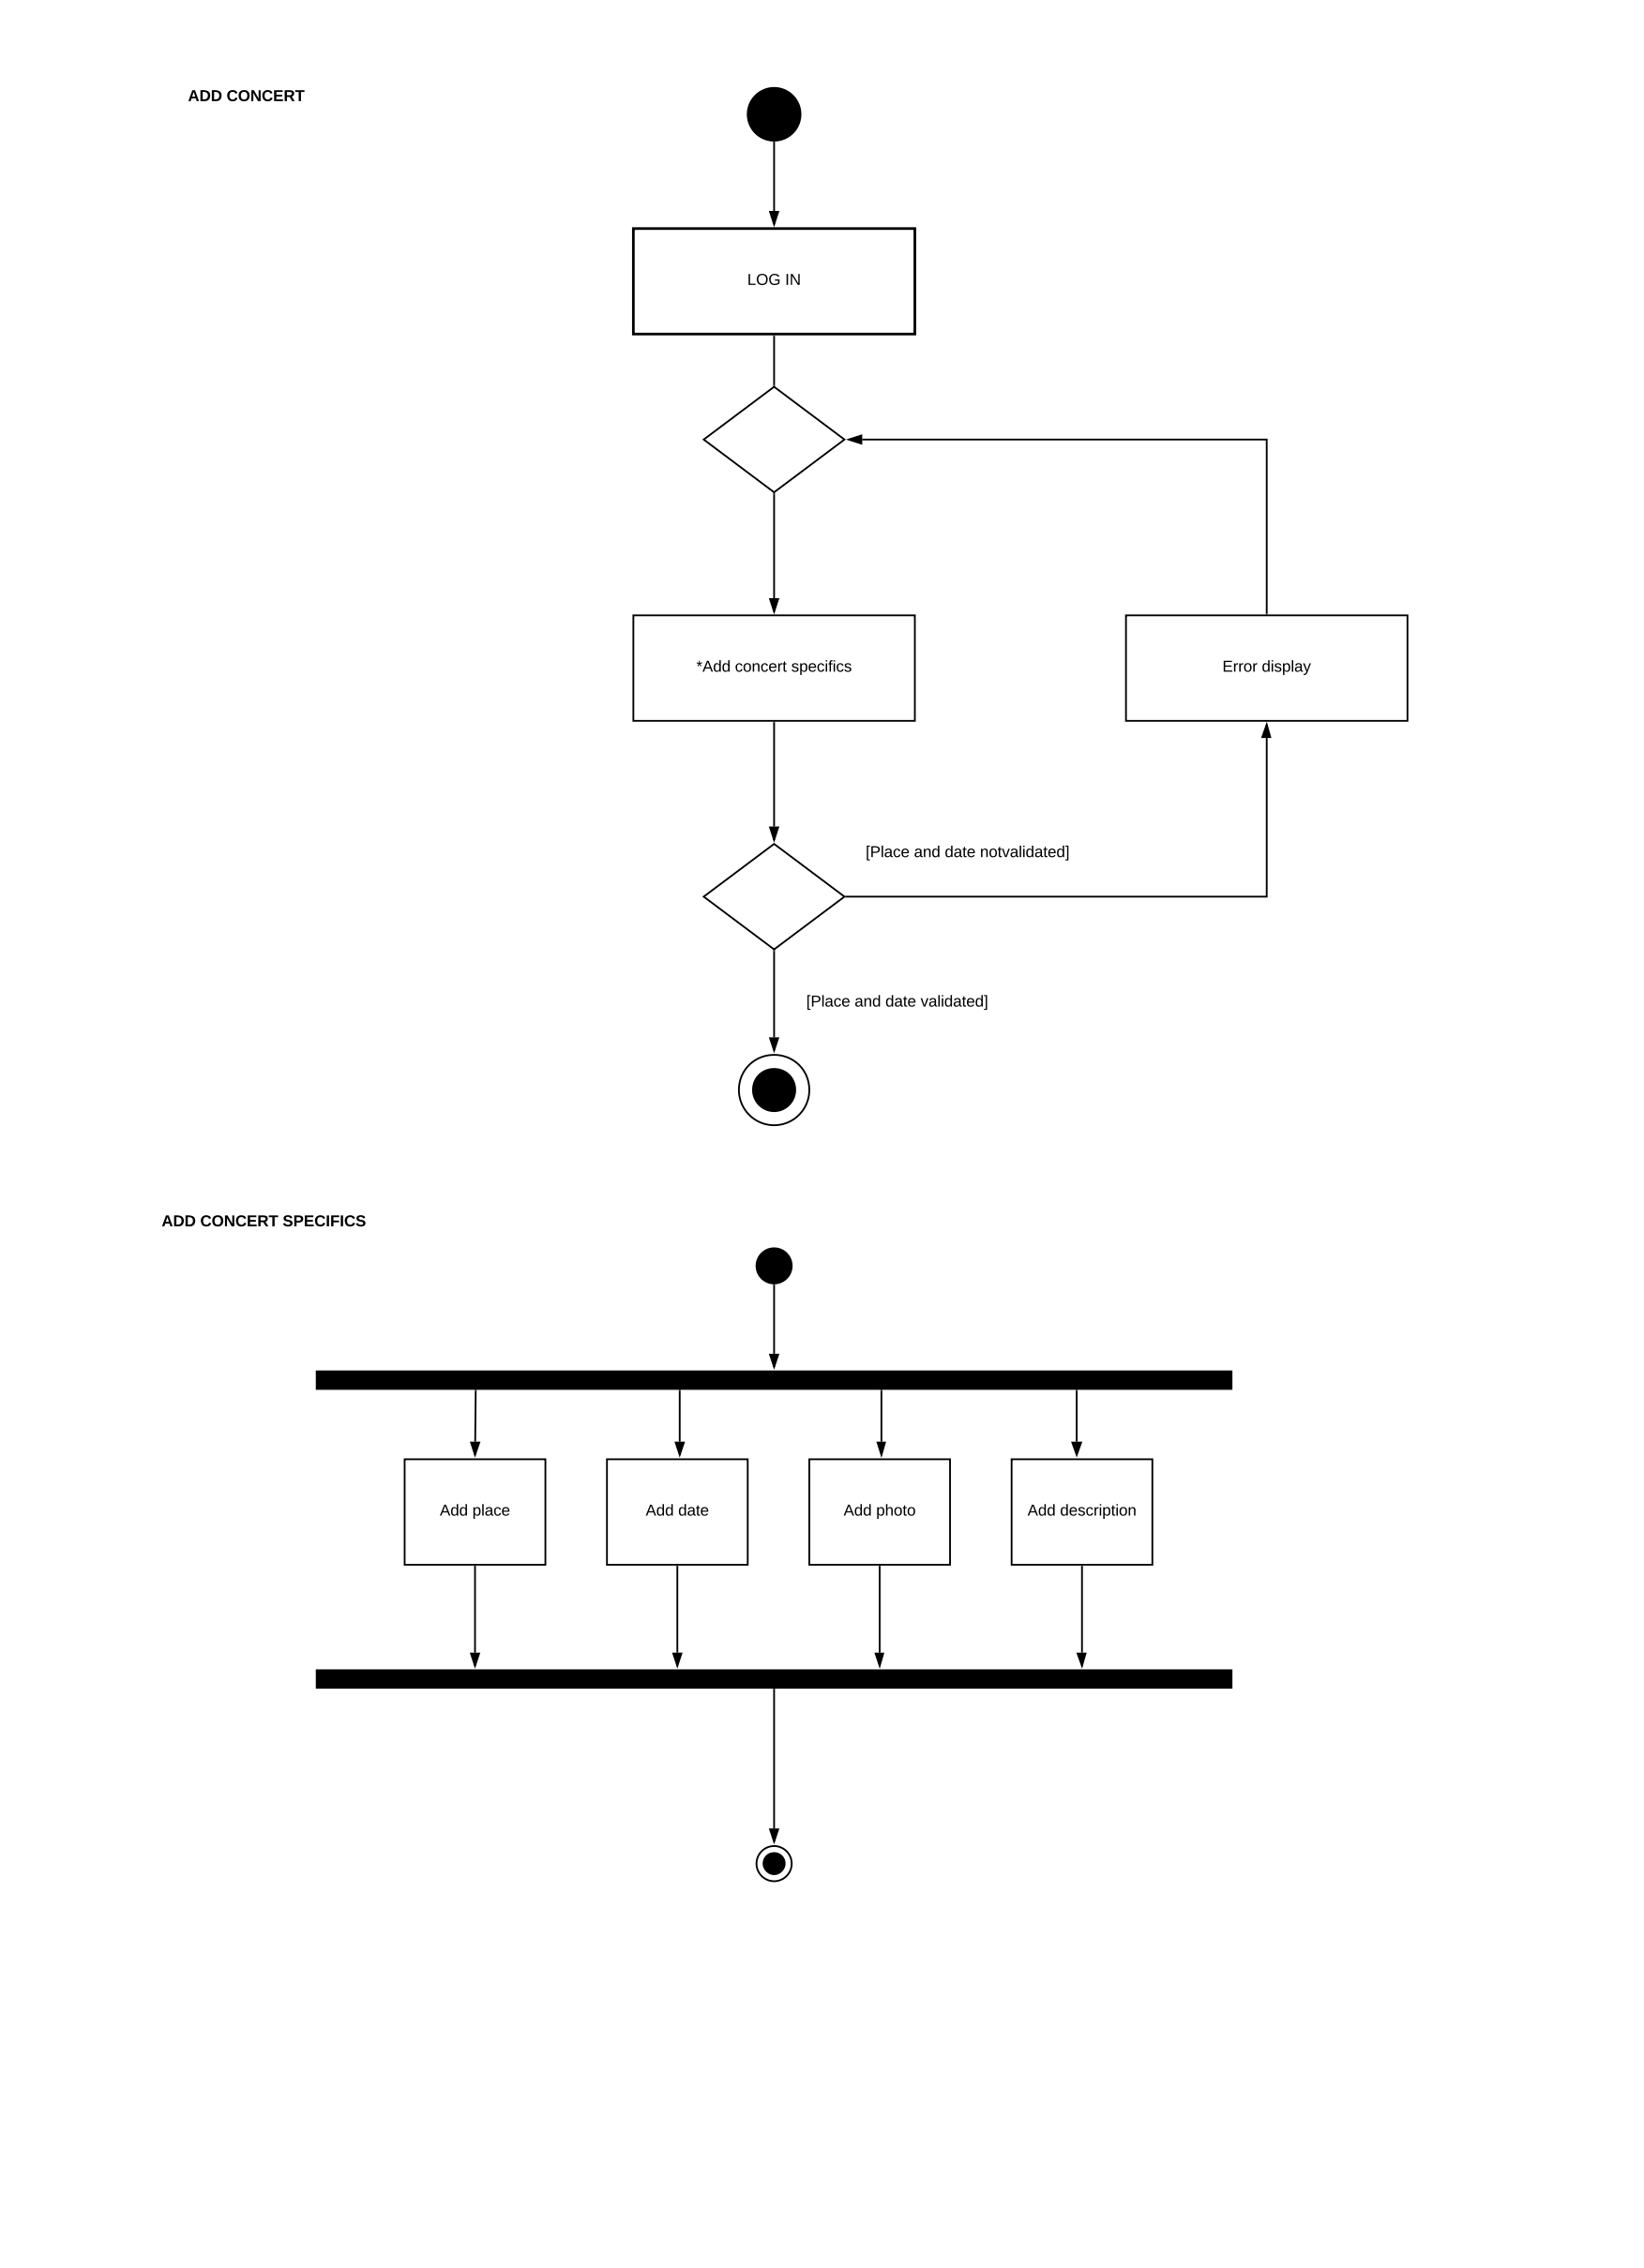
\includegraphics[scale=0.5]{addconcertdiagram.jpg}
\subsection{Ferrarelli}
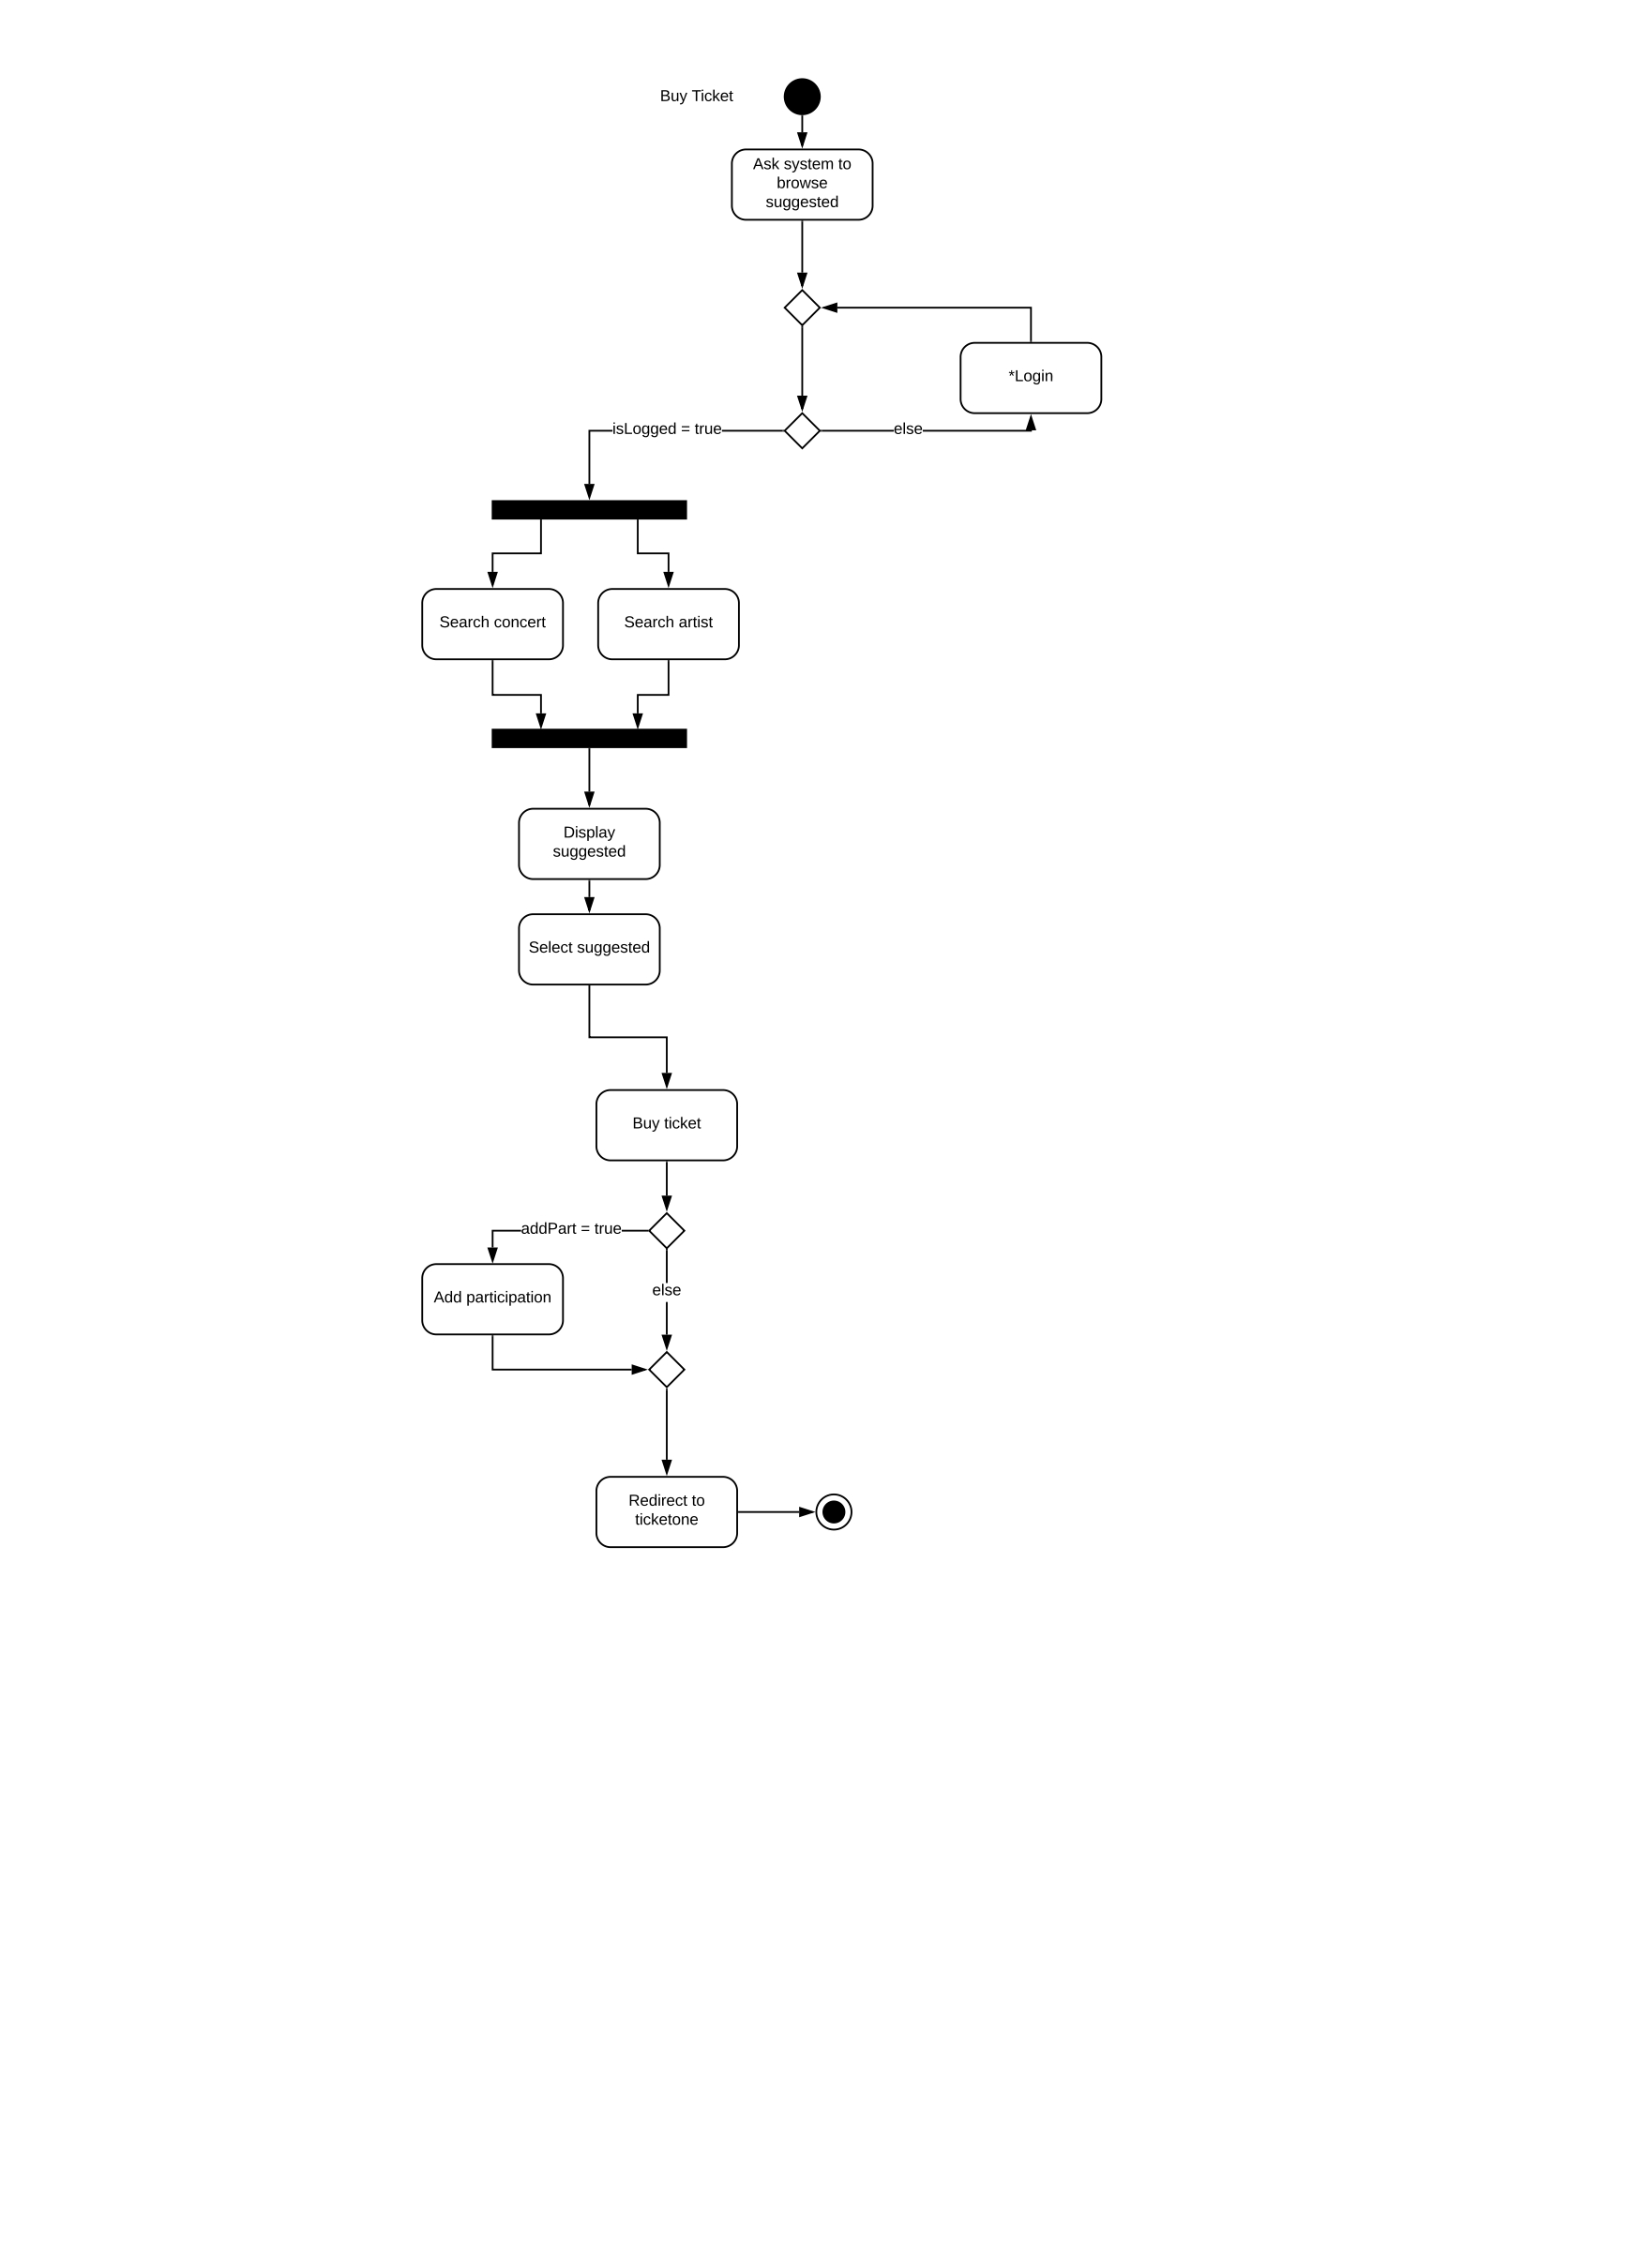
\includegraphics[scale=0.5]{hmwActivityDiagram.jpg}
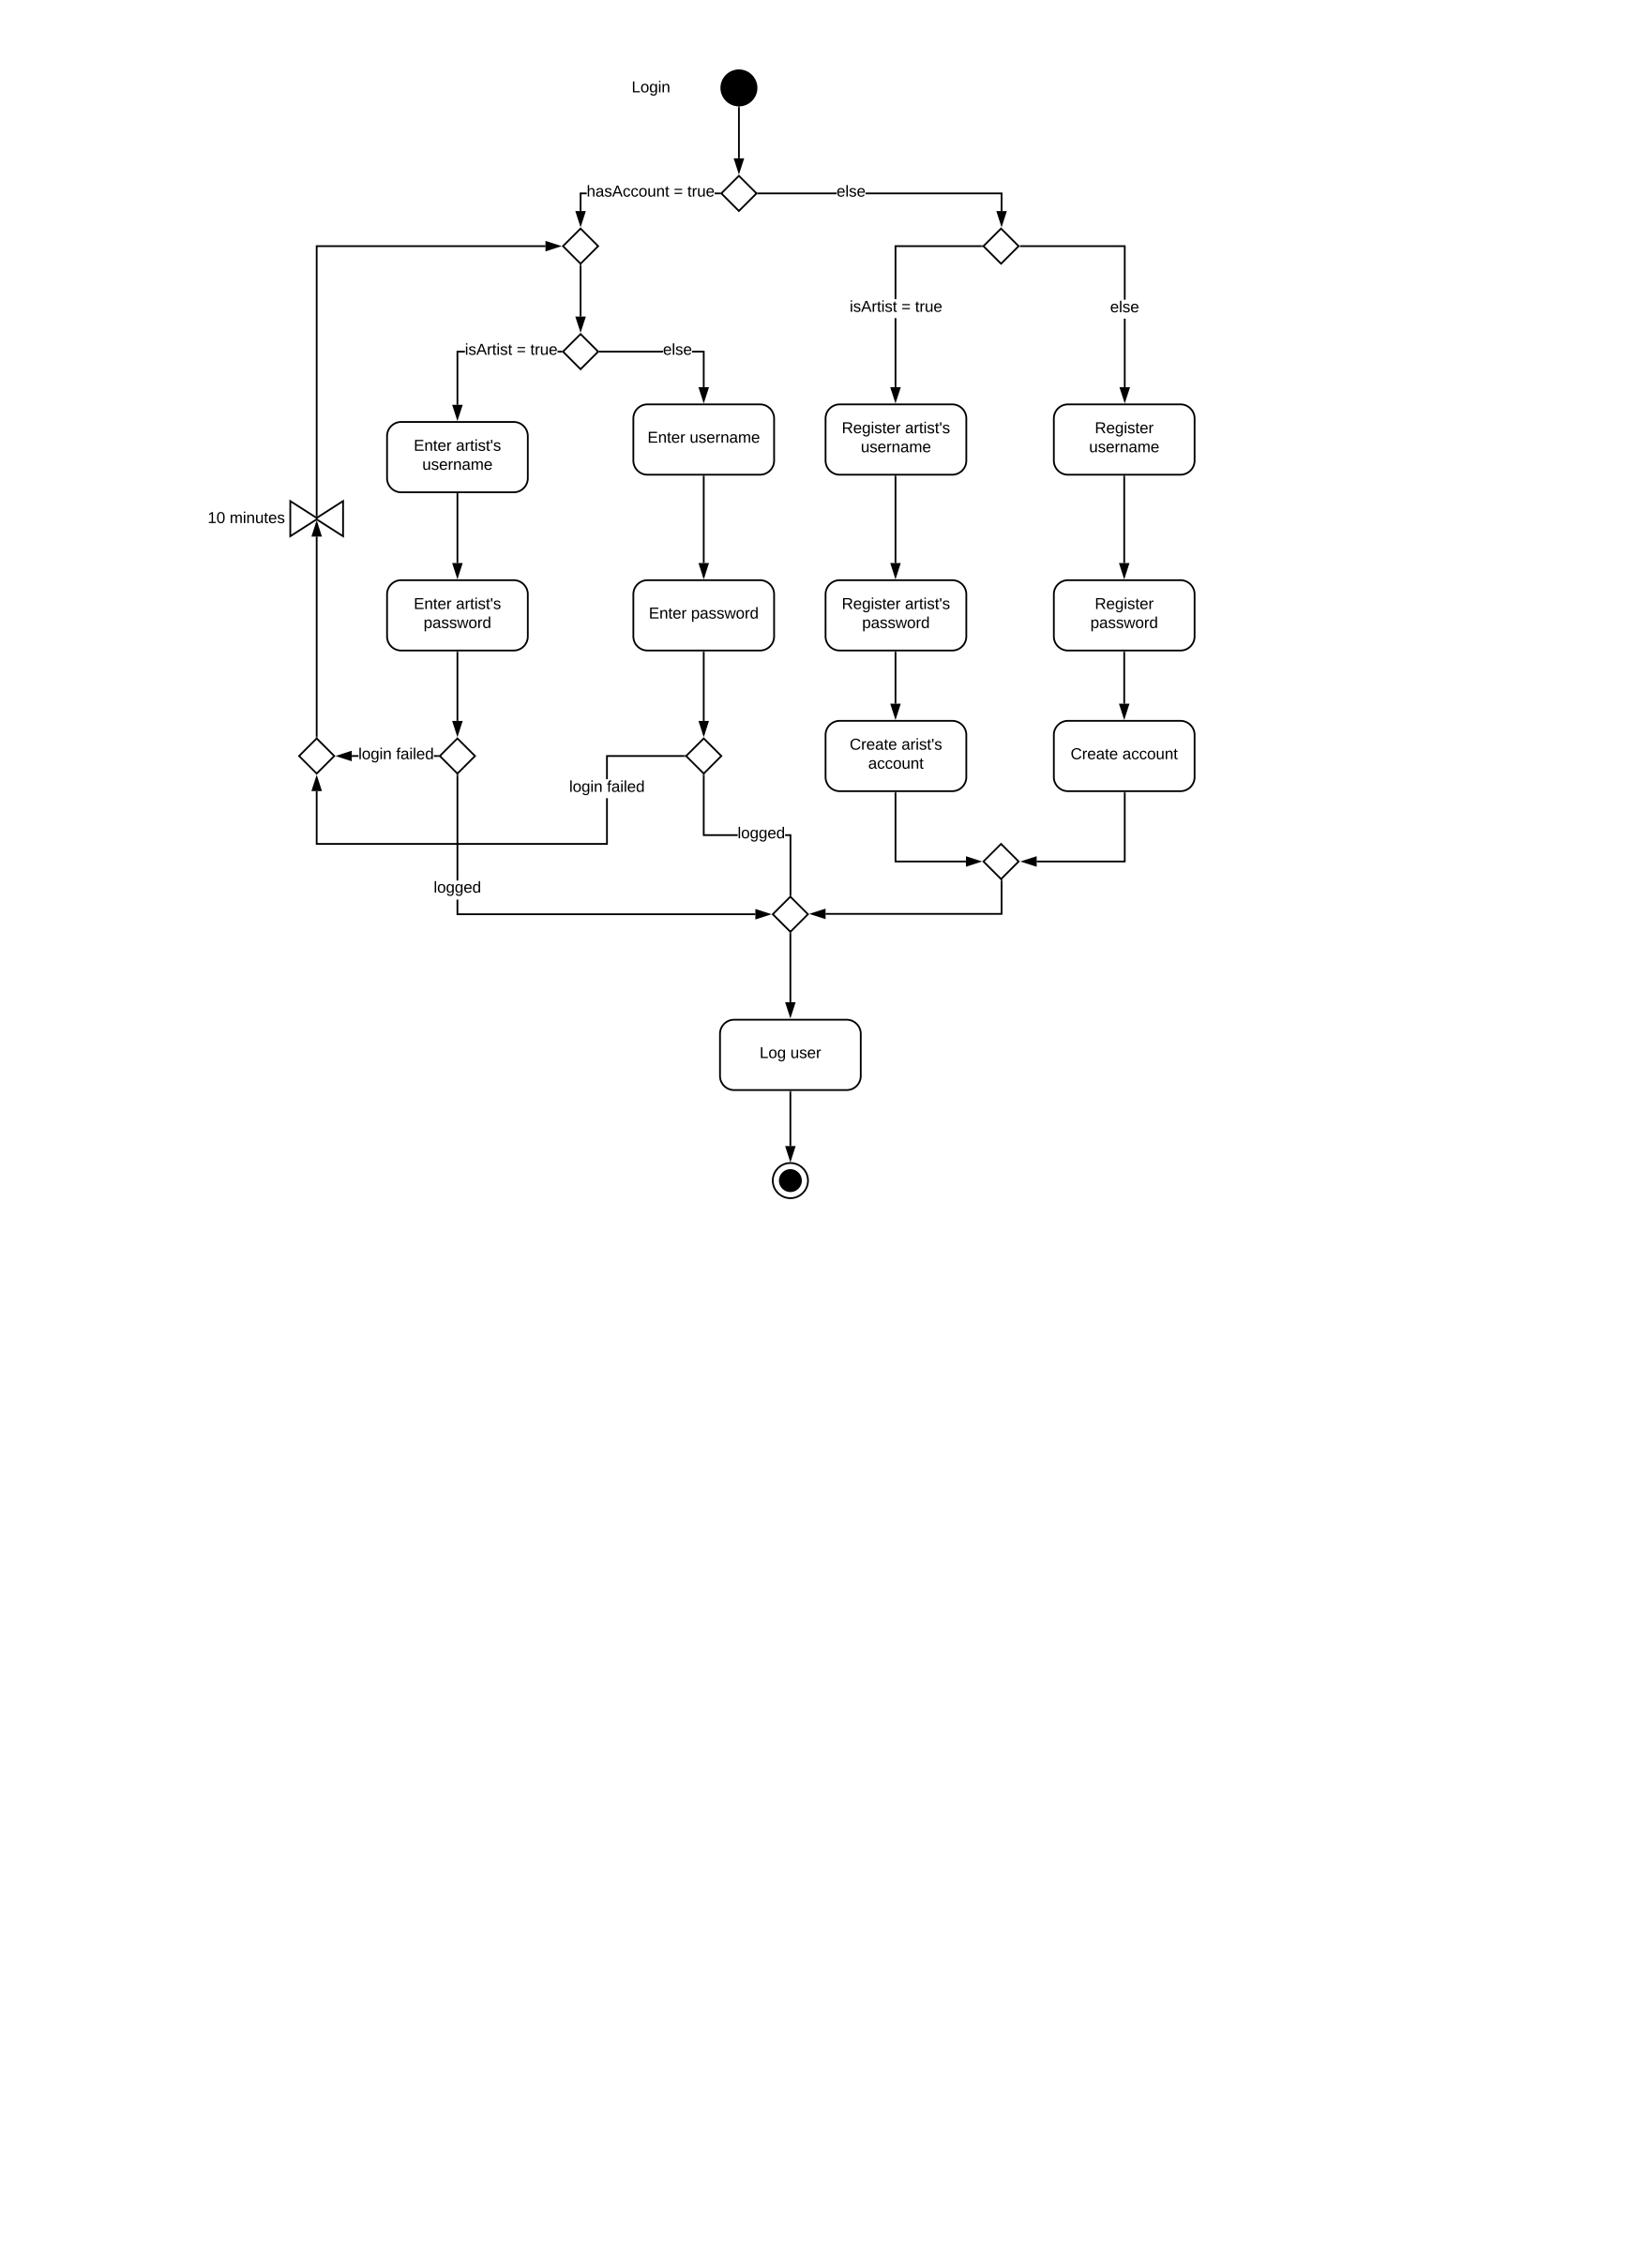
\includegraphics[scale=0.5]{logActivityDiagram.jpg}
\subsection{Ferri}
\section{SonarCloud}
\paragraph{SonarCloud link} https://sonarcloud.io/organizations/ferra-rally/projects
\end{itemize}
\end{document}